%! TEX program = xelatex
%% \documentclass[letterpaper,nonstop,draftmode]{simplethesisdissertation}
\documentclass[12pt,twoside]{report}
%!TEX root = ./Thesis.tex
\usepackage{breakcites}
\usepackage{amsmath,amssymb}
\usepackage{amsfonts}
\usepackage{mathtools}

\usepackage{blindtext} % Package to generate dummy text throughout this template 

%%%%%%%%%%%%%%%%%% FONT CHOICE %%%%%%%%%%%%%%%%%%%%%%

% \usepackage{unicode-math}
\usepackage[bold-style=ISO]{unicode-math}
\usepackage{parskip}
\defaultfontfeatures{Scale=MatchLowercase}
\setmainfont{TeX Gyre Pagella}[Scale = 1.0]

% \setmathfont{Pagella Math}
% \setmathfont{XITS Math}
\usepackage{bm}

% \renewcommand{\boldsymbol}{\symbf} % this is because unicode-math with the bold-style option wants you to use \symbf rather that \boldsymbol, for some reason

% \linespread{1.05} % Line spacing - Palatino needs more space between lines

%%%%%%%%%%%%%%%%%% END FONT CHOICE %%%%%%%%%%%%%%%%%%%%%%

\usepackage{xspace} % to avoid newcommand eating trailing space
\usepackage{etoolbox}
\usepackage{microtype} % Slightly tweak font spacing for aesthetics

\usepackage[english]{babel} % Language hyphenation and typographical rules

\usepackage[hmarginratio=1:1,top=32mm,columnsep=20pt]{geometry} % Document margins
\usepackage{marginnote}
\renewcommand*{\marginfont}{\color{blue}\itshape\footnotesize}
\usepackage{setspace} % provides \setstretch
\usepackage[small,labelfont=bf,up,textfont=it,up]{caption} % Custom captions under/above floats in tables or figures
\usepackage{subcaption}
\usepackage{booktabs} % Horizontal rules in tables
\usepackage{fullpage}

\usepackage{lettrine} % The lettrine is the first enlarged letter at the beginning of the text

\usepackage{enumitem} % Customized lists
\setlist[itemize]{noitemsep} % Make itemize lists more compact


\usepackage{acronym}
\newacro{AD}{Automatic Differentiation}
\newacro{DR}{Dimensionality Reduction}
\newacro{ML}{Machine Learning}
\newacro{NN}{Neural Network}
\newacro{PCA}{Principal Component Analysis}
\newacro{CNN}{Convolutional Neural Network}
\newacro{SGD}{Stochastic Gradient Descend}
\newacro{SVM}{Support Vector Machine}
\newacro{QFT}{Quantum Fourier Transform}
\newacro{QML}{Quantum Machine Learning}

\newacro{QW}{Quantum Walk}
\newacro{DTQW}{Discrete-Time Quantum Walk}
\newacro{CTQW}{Continuous-Time Quantum Walk}

\newacro{LG}{Laguerre-Gauss}
\newacro{CCD}{Charge Coupled Device}
\newacro{SLM}{Spatial Light Modulator}
\newacro{SAM}{Spin Angular Momentum}
\newacro{OAM}{Orbital Angular Momentum}
\newacro{QWP}{Quarter-Wave Plate}
\newacro{HWP}{Half-Wave Plate}
\newacro{VVB}{Vector Vortex Beam}
\newacro{PBS}{Polarising Beamsplitter}
\newacro{QP}{Q-Plate}
\newacro{SMF}{Single Mode Optical Fiber}
\newacro{APD}{Avalanche Photodiode}
\newacro{SCS}{Spin Coherent State}
\newacro{SPDC}{Spontaneous Parametric Down Conversion}
\newacro{PPKTP}{Periodically-Poled Potassium Titanyl Phosphate}

\usepackage{todonotes}

\usepackage{abstract} % Allows abstract customization
\renewcommand{\abstractnamefont}{\normalfont\bfseries} % Set the "Abstract" text to bold
\renewcommand{\abstracttextfont}{\normalfont\small\itshape} % Set the abstract itself to small italic text

% \usepackage{titlesec} % Allows customization of titles
% \renewcommand\thesection{\Roman{section}} % Roman numerals for the sections
% \renewcommand\thesubsection{\roman{subsection}} % roman numerals for subsections
% \titleformat{\section}[block]{\large\scshape\centering}{\thesection.}{1em}{} % Change the look of the section titles
% \titleformat{\subsection}[block]{\large}{\thesubsection.}{1em}{} % Change the look of the section titles

% \usepackage{fancyhdr} % Headers and footers
% \pagestyle{fancy} % All pages have headers and footers
% \fancyhead{} % Blank out the default header
% \fancyfoot{} % Blank out the default footer
% \fancyhead[C]{Running title $\bullet$ May 2016 $\bullet$ Vol. XXI, No. 1} % Custom header text
% \fancyfoot[RO,LE]{\thepage} % Custom footer text

\usepackage{titling} % Customizing the title section

\usepackage{physics}
\usepackage{siunitx}

\usepackage{csquotes}

\usepackage{easyReview}

\usepackage{graphicx}
\graphicspath{{./Figures/}{./Figures/gate-learning/}{./Figures/quantum-walks/}{./Figures/VVBs/}}
\usepackage{wrapfig}
% \usepackage{subfig}

\usepackage{placeins}  % provides \FloatBarrier

\usepackage{xcolor}
\usepackage{nameref}
\usepackage[colorlinks=true,citecolor=red]{hyperref}
\usepackage[nameinlink]{cleveref}
\crefname{appsec}{Appendix}{Appendices}

\usepackage{listings} % for code snippets
\definecolor{codegreen}{rgb}{0,0.6,0}
\definecolor{codegray}{rgb}{0.5,0.5,0.5}
\definecolor{codepurple}{rgb}{0.58,0,0.82}
\definecolor{backcolour}{rgb}{0.95,0.95,0.92}
 
\lstdefinestyle{mystyle}{
    backgroundcolor=\color{backcolour},
    commentstyle=\color{codegreen},
    keywordstyle=\color{magenta},
    numberstyle=\tiny\color{codegray},
    stringstyle=\color{codepurple},
    basicstyle=\ttfamily\scriptsize,
    breakatwhitespace=false,
    breaklines=true,
    captionpos=b,
    keepspaces=true,
    numbers=left,
    numbersep=5pt,
    showspaces=false,
    showstringspaces=false,
    showtabs=false,
    tabsize=2
} 
\lstset{style=mystyle}


\usepackage{tikz}

\usepackage{amsthm}
% \newtheorem{example}{Example}

\usepackage[many]{tcolorbox}
% \tcbuselibrary{theorems}
% \newtcbtheorem
%   [number within=section]% init options
%   {example}% name
%   {Example}% title
%   {%
%     breakable, enhanced,
%     colback=green!5,
%     colframe=green!35!black,
%     fonttitle=\bfseries,
%     title={Porco dio}
%   }% options
%   {example}% prefix
\newtcolorbox[
    auto counter,
    number within=section,
    crefname={example}{examples}
]{example}[1][]{
  enhanced,
  breakable,
%   colback=green!5,
%   colframe=green!35!black,
  fonttitle=\bfseries,
  title={Example \thetcbcounter},
  #1
}

\newtcolorbox[
    auto counter,
    number within=section,
    crefname={example}{examples}
]{examplebox}[2][]{
  enhanced,
  breakable,
  fonttitle=\bfseries,
  title={Example \thetcbcounter: #2},
  #1
}

\newtcolorbox[auto counter]{tbox}[2][]{%
	enhanced,% float*=t,
	colback=gray!5!white, colframe=gray!75!black,
	width=\textwidth,
	title={Box \thetcbcounter: #2}, #1
}


% \usepackage[
%     backend=biber,
%     style=alphabetic,
%     maxcitenames=1,
%     url=true,
%     doi=true,
%     sorting=ynt,
%     backref=true
% ]{biblatex}
% \DeclareNameAlias{author}{given-family}

\usepackage{breakcites}
\usepackage[
    backend=biber,
    style=authoryear,
    maxnames=1,
    url=false,
    doi=true,
    sortcites=true,
    sorting=ynt,
    backref=true,
    firstinits=false,
    uniquelist=false, % to suppress multiple author names being used
    uniquename=false,
    % nohashothers=true, nosortothers=true,
    natbib
]{biblatex}
\renewcommand{\cite}{\parencite}


\DeclareNameFormat{labelname}{%
  \ifcase\value{uniquename}%
    \usebibmacro{name:family}
      {\namepartfamily}
      {\namepartgiven}
      {\namepartprefix}
      {\namepartsuffix}%
  \or
    \ifuseprefix
      {\usebibmacro{name:given-family}
        {\namepartfamily}
        {\namepartgiveni}
        {\namepartprefix}
        {\namepartsuffixi}}
      {\usebibmacro{name:given-family}
        {\namepartfamily}
        {\namepartgiveni}
        {\namepartprefixi}
        {\namepartsuffixi}}%
  \or
    \usebibmacro{name:given-family}
      {\namepartfamily}
      {\namepartgiven}
      {\namepartprefix}
      {\namepartsuffix}%
  \fi}


% ---------------- START SECOND FIX


\ExecuteBibliographyOptions{maxcitenames=1}

\DeclareFieldFormat{citehyperref}{%
  \DeclareFieldAlias{bibhyperref}{noformat}% Avoid nested links
  \bibhyperref{#1}}

\DeclareFieldFormat{textcitehyperref}{%
  \DeclareFieldAlias{bibhyperref}{noformat}% Avoid nested links
  \bibhyperref{%
    #1%
    \ifbool{cbx:parens}
      {\bibcloseparen\global\boolfalse{cbx:parens}}
      {}}}

\savebibmacro{cite}
\savebibmacro{textcite}

\renewbibmacro*{cite}{%
  \printtext[citehyperref]{%
    \restorebibmacro{cite}%
    \usebibmacro{cite}}}

\renewbibmacro*{textcite}{%
  \ifboolexpr{
    ( not test {\iffieldundef{prenote}} and
      test {\ifnumequal{\value{citecount}}{1}} )
    or
    ( not test {\iffieldundef{postnote}} and
      test {\ifnumequal{\value{citecount}}{\value{citetotal}}} )
  }
    {\DeclareFieldAlias{textcitehyperref}{noformat}}
    {}%
  \printtext[textcitehyperref]{%
    \restorebibmacro{textcite}%
    \usebibmacro{textcite}}}

% ---------------- END SECOND FIX

\usepackage{xparse,xcoffins}

\ExplSyntaxOn
\NewCoffin\imagecoffin
\NewCoffin\labelcoffin

\keys_define:nn { miguel/label }
 {
  label   .tl_set:N = \l_miguel_label_tl,
  labelbox .bool_set:N = \l_miguel_label_box_bool,
  labelbox .default:n = true,
  fontsize .tl_set:N = \l_miguel_label_size_tl,
  fontsize .initial:n = \footnotesize,
  pos .choice:,
  pos/nw .code:n = \tl_set:Nn \l_miguel_label_pos_tl { left,up },
  pos/ne .code:n = \tl_set:Nn \l_miguel_label_pos_tl { right,up },
  pos/sw .code:n = \tl_set:Nn \l_miguel_label_pos_tl { left,down },
  pos/se .code:n = \tl_set:Nn \l_miguel_label_pos_tl { right,down },
  pos/n .code:n = \tl_set:Nn \l_miguel_label_pos_tl { hc,up },
  pos/w .code:n = \tl_set:Nn \l_miguel_label_pos_tl { left,vc },
  pos/s .code:n = \tl_set:Nn \l_miguel_label_pos_tl { hc,down },
  pos/e .code:n = \tl_set:Nn \l_miguel_label_pos_tl { right,vc },
  pos .initial:n = nw,
  unknown .code:n   = \clist_put_right:Nx \l_miguel_label_clist
                       { \l_keys_key_tl = \exp_not:n { #1 } }
 }
\clist_new:N \l_miguel_label_clist
\box_new:N \l_miguel_label_box
\box_new:N \l_miguel_label_image_box

\NewDocumentCommand{\xincludegraphics}{O{}m}
 {
  \group_begin:
  \tl_clear:N \l_miguel_label_tl
  \clist_clear:N \l_miguel_label_clist
  \keys_set:nn { miguel/label } { #1 }
  \tl_if_empty:NTF \l_miguel_label_tl
   {
    \miguel_includegraphics:Vn \l_miguel_label_clist { #2 }
   }
   {
    \SetHorizontalCoffin\imagecoffin
     {
      \miguel_includegraphics:Vn \l_miguel_label_clist { #2 }
     }
    \SetHorizontalCoffin\labelcoffin
     {
      \raisebox{\depth}
       {
        \bool_if:NTF \l_miguel_label_box_bool
         { \fcolorbox{white}{white}{\l_miguel_label_size_tl\l_miguel_label_tl} }
         { \l_miguel_label_size_tl\l_miguel_label_tl }
       }
     }
    \SetVerticalPole\imagecoffin{left}{3pt+\CoffinWidth\labelcoffin/2}
    \SetVerticalPole\imagecoffin{right}{\Width-3pt-\CoffinWidth\labelcoffin/2}
    \SetHorizontalPole\imagecoffin{up}{\Height-3pt-\CoffinHeight\labelcoffin/2}
    \SetHorizontalPole\imagecoffin{down}{3pt+\CoffinHeight\labelcoffin/2}
    \use:x{\JoinCoffins\imagecoffin[\l_miguel_label_pos_tl]\labelcoffin[vc,hc]} 
    \TypesetCoffin\imagecoffin
   }
   \group_end:
 }
\NewDocumentCommand{\setlabel}{m}
 {
  \keys_set:nn { miguel/label } { #1 }
 }

\cs_new_protected:Nn \miguel_includegraphics:nn
 {
  \includegraphics[#1]{#2}
 }
\cs_generate_variant:Nn \miguel_includegraphics:nn { V }

\ExplSyntaxOff

\addbibresource{Thesis.bib}


\newcommand{\bs}[1]{\pmb{#1}}
\newcommand{\on}[1]{\operatorname{#1}}

\newcommand{\bsx}{\bs{x}}
\newcommand{\bslambda}{{\bs{\lambda}}}
\renewcommand{\grad}{\nabla}

\newcommand{\calA}{{\mathcal{A}}}
\newcommand{\calC}{{\mathcal{C}}}
\newcommand{\calE}{{\mathcal{E}}}
\newcommand{\calF}{{\mathcal{F}}}
\newcommand{\calG}{{\mathcal{G}}}
\newcommand{\calH}{{\mathcal{H}}}
\newcommand{\calP}{{\mathcal{P}}}
\newcommand{\calS}{{\mathcal{S}}}
\newcommand{\calU}{{\mathcal{U}}}
\newcommand{\calW}{{\mathcal{W}}}
\newcommand{\calV}{{\mathcal{V}}}

\newcommand{\calHcoin}{{\calH_\calC}}
\newcommand{\calHwalker}{{\calH_\calS}}

\newcommand{\barF}{\bar{\calF}}

\newcommand{\CC}{\mathbb{C}}
\newcommand{\EE}{\mathbb{E}}
\newcommand{\HH}{\mathbb{H}}
\newcommand{\NN}{\mathbb{N}}
\newcommand{\PP}{\mathbb{P}}
\newcommand{\QQ}{\mathbb{Q}}
\newcommand{\RR}{\mathbb{R}}
\newcommand{\ZZ}{\mathbb{Z}}

\newcommand{\tildePP}{\tilde{\PP}}

\newcommand{\UToff}{\calU_{\on{Toff}}}
\newcommand{\HToff}{\calH_{\on{Toff}}}
\newcommand{\HPrimeToff}{\calH'_{\on{Toff}}}
\newcommand{\HTildeToff}{\tilde{\calH}_{\on{Toff}}}

\newcommand{\UFred}{\calU_{\Fred}}
\newcommand{\Fred}{\on{Fred}}
\newcommand{\HFred}{\calH_{\Fred}}
\newcommand{\HTildeFred}{\tilde{\calH}_{\Fred}}
\newcommand{\HPrimeFred}{\calH'_{\Fred}}

\newcommand{\CNOT}{\on{CNOT}}
\newcommand{\Toff}{\on{Toff}}

\newcommand{\spanR}{\on{Span}_{\RR}}

\DeclareMathOperator*{\argmax}{arg\,max}
\DeclareMathOperator*{\argmin}{arg\,min}
\DeclareMathOperator*{\Prob}{Prob}

\newcommand{\barcalF}{\overline{\calF}}

\newcommand{\Lin}{\on{Lin}}

\newcommand\scalemath[2]{\scalebox{#1}{\mbox{\ensuremath{\displaystyle #2}}}}



% \usepackage{fancyhdr}

%%%%%%%%%%%%%%%%%%%%%%%%%%%%%%%%%%%%%%%%%%%%%%%%%%%%%%%%%%%%%%%%%
%% PREAMBLE.
%%%%%%%%%%%%%%%%%%%%%%%%%%%%%%%%%%%%%%%%%%%%%%%%%%%%%%%%%%%%%%%%%

% Document properties.
\def\DocumentTitle{Machine-learning-assisted state and gate engineering for quantum technologies}
\def\AuthorName{Luca Innocenti}

% PDF settings and properties.
\hypersetup{
pdftitle={\DocumentTitle},
pdfauthor={\AuthorName},
pdfsubject={Ph.D. Thesis, Queen's University Belfast, 2019},
pdfcreator={XeLaTeX},
pdfproducer={},
pdfkeywords={},
unicode=true,
% bookmarks=true,
bookmarksopen=true,
pdfstartview=FitH,
pdfpagelayout=OneColumn,
pdfpagemode=UseOutlines,
hidelinks,
breaklinks,
bookmarksnumbered
}
\hypersetup{
  colorlinks   = true, %Colours links instead of ugly boxes
  urlcolor     = green!80!black, %Colour for external hyperlinks
  linkcolor    = blue, %Colour of internal links 	q
  citecolor    = red!80!black %Colour of citations
}

% Accent colors.
\definecolor{AccentOne}{RGB}{0,68,186} % blue

%%%%%%%%%%%%%%%%%%%%%%%%%%%%%%%%%%%%%%%%%%%%%%%%%%%%%%%%%%%%%%%%%
%% ACTUAL DOCUMENT.
%%%%%%%%%%%%%%%%%%%%%%%%%%%%%%%%%%%%%%%%%%%%%%%%%%%%%%%%%%%%%%%%%

% \pagestyle{fancy}
% \fancyhf{}
% \fancyhead[LE,RO]{Overleaf}
% \fancyhead[RE,LO]{Guides and tutorials}
% \fancyfoot[CE,CO]{\leftmark}
% \fancyfoot[LE,RO]{\thepage}

% \usepackage{comment}
% \excludecomment{figure}
% \let\endfigure\relax


\begin{document}

%!TEX root = ./Thesis.tex

% Use Roman numerals (i, ii, iii, etc.) for page numbers in the front matter.
\pagenumbering{roman}

%%%%%%%%%%%%%%%%%%%%%%%%%%%%%%%%%%%%%%%%%%%%%%%%%%%%%%%%%%%%%%%%%
%% TITLE PAGE.
%%%%%%%%%%%%%%%%%%%%%%%%%%%%%%%%%%%%%%%%%%%%%%%%%%%%%%%%%%%%%%%%%

% No headers or footers on the title page.
\thispagestyle{empty}

\begingroup

\centering{
    \includegraphics[width=0.5\columnwidth]{Figures/logo.jpg}} \par
\centering
\setstretch{1.0}
~
\\[1em]
\sffamily\bfseries\fontsize{26}{31.2}\selectfont
\DocumentTitle
% \\
% Use Manual Line Breaks If Necessary
\\[0.4in]
\normalfont\large
Thesis submitted for the degree of
\\[0.25em]
{\itshape Doctor of Philosophy}
\\[0.25em]
in the
\\[0.25em]
Faculty of Engineering and Physical Sciences
\\[0.25em]
by
\\[0.25em]
\sffamily\bfseries\Large
\AuthorName
\\[0.4in]
\normalfont\normalsize
% In Partial Fulfillment of the Requirements
% \\[0.5em]
% for the Degree of
% \\[0.5em]
% Doctor of Philosophy
% \\[0.5em]
% in
% \\[0.5em]
% Physics
\vfill
% \includegraphics[height=1.8in]
% {Figure-SchoolLogo}
% \\[1.5em]
School of Mathematics and Physics
\\[0.5em]
Queen's University Belfast
\\[0.5em]
% Belfast, UK
% \\[1.5em]
% 2020
% \\[0.5em]
\emph{\textbf{May 2020}}
\par
\endgroup

\clearpage

%%%%%%%%%%%%%%%%%%%%%%%%%%%%%%%%%%%%%%%%%%%%%%%%%%%%%%%%%%%%%%%%%
%% COPYRIGHT PAGE.
%%%%%%%%%%%%%%%%%%%%%%%%%%%%%%%%%%%%%%%%%%%%%%%%%%%%%%%%%%%%%%%%%

\pagestyle{plain}
\setcounter{page}{2}

\begingroup
\centering
\setstretch{1.0}
\null
\vfill
{\sffamily\textcopyright}~2020
\\[0.5em]
\AuthorName
\\[0.5em]
All Rights Reserved
\par
\endgroup

\clearpage

%%%%%%%%%%%%%%%%%%%%%%%%%%%%%%%%%%%%%%%%%%%%%%%%%%%%%%%%%%%%%%%%%
%% DEDICATION PAGE.
%%%%%%%%%%%%%%%%%%%%%%%%%%%%%%%%%%%%%%%%%%%%%%%%%%%%%%%%%%%%%%%%%

% \begingroup
% \centering
% \setstretch{1.0}
% ~
% \\[1in]
% \textit{Insert dedication here}
% \par
% \endgroup

\clearpage

%%%%%%%%%%%%%%%%%%%%%%%%%%%%%%%%%%%%%%%%%%%%%%%%%%%%%%%%%%%%%%%%%
%% ACKNOWLEDGMENTS.
%%%%%%%%%%%%%%%%%%%%%%%%%%%%%%%%%%%%%%%%%%%%%%%%%%%%%%%%%%%%%%%%%

\chapter*{Acknowledgments}
% \addcontentsline{toc}{chapter}{Acknowledgments}
My gratitude goes to every member of QTeQ, current and past, that I had the pleasure to interact with, but first and foremost to Mauro, for his unwavering support, and for making the whole thing possible in the first place. To Mauro and Alessandro, for enduring me through countless meetings and discussions, and always being helpful.
To Chiara, for bearing with me throughout these years.
In loose chronological order, to Gabriele, Steve, Matteo, Christine, Helena, Darren, Obinna, Oussama, Qiongyuan, Adam, Peter, Hannah, Giorgio, Marta, Ricardo, Eoghan, Luca, Alessio, and everyone else currently quarantined who knows where in the world.
See you at 4pm.


\clearpage

%%%%%%%%%%%%%%%%%%%%%%%%%%%%%%%%%%%%%%%%%%%%%%%%%%%%%%%%%%%%%%%%%
%% ABSTRACT.
%%%%%%%%%%%%%%%%%%%%%%%%%%%%%%%%%%%%%%%%%%%%%%%%%%%%%%%%%%%%%%%%%

\chapter*{Abstract}
\addcontentsline{toc}{chapter}{Abstract}

In this Thesis, we discuss applications of machine learning to quantum information science.
The interface between these two fields has been the subject of much research, recently, driven by the many successes of machine learning for diverse pattern recognition tasks. The work reported in this Thesis addresses precisely the potential of such an interdisciplinary line of research and illustrates how machine learning provides a valuable add-on to standard techniques used in the context of quantum technologies.

Specifically, we will first study the problem of devising time-independent dynamics implementing target quantum operations.
This involves a challenging optimisation task, which is hard to tackle with standard numerical tools.
We demonstrate how the use of supervised learning algorithms can dramatically speed-up this task.

We then consider the tasks of engineering and characterising quantum states in large Hilbert spaces. Motivated by strong experimental reasons, we consider explicitly the embodiment of such multi-dimensional quantum systems provided by the orbital angular momentum and polarisation degrees of freedom of light.
We devise a protocol involving quantum walks to implement arbitrary states by only making use of the possibility to couple polarisation and orbital angular momentum through relatively recent technological advances in the field of linmear optics.
This protocol relies solely on the properties of quantum walk dynamics, and is therefore applicable to different types of architectures.

We then present an experimental demonstration of this engineering strategy, and consider the issue of assessing the quality of the states thus generated.
We show how different machine learning algorithms, including supervised and unsupervised learning ones, are able to tackle this problem and provide useful information in realistic experimental conditions.

% \chapter*{Note}
% {\HUGE Fuck you}
% {\Huge Note:}
% \vfill
% {\large\bfseries Note:}
% To provide further structure to the thesis, paragraph headings are used to give the reader a quick idea of what that is addressed in that section of text \highlight{(ugh)}.


\clearpage

%%%%%%%%%%%%%%%%%%%%%%%%%%%%%%%%%%%%%%%%%%%%%%%%%%%%%%%%%%%%%%%%%
%% TABLE OF CONTENTS (TOC), LISTS OF FIGURES, TABLES, ETC.
%%%%%%%%%%%%%%%%%%%%%%%%%%%%%%%%%%%%%%%%%%%%%%%%%%%%%%%%%%%%%%%%%

\tableofcontents

% \listoffigures

% \listoftables

\clearpage

% Use Arabic numerals (1, 2, 3, etc.) for subsequent page numbers.
\pagenumbering{arabic}


{\renewcommand{\bibname}{List of publications}
\begin{thebibliography}{9}

\bibitem{QWengineering} 
Luca Innocenti, Helena Majury, Taira Giordani, Nicolò Spagnolo, Fabio Sciarrino, Mauro Paternostro, and Alessandro Ferraro. ``Quantum state engineering using one-dimensional discrete-time quantum walks''. In \emph{Physical Review A} 96, 062326. {\footnotesize\scshape DOI:} \href{https://doi.org/10.1103/PhysRevA.96.062326}{10.1103/PhysRevA.96.062326}. arXiv: \href{https://arxiv.org/abs/1710.10518}{1710.10518 [quant-ph]} (2017).

\bibitem{gatelearning} 
Luca Innocenti, Leonardo Banchi, Alessandro Ferraro, Sougato Bose, and Mauro Paternostro. ``Supervised learning of time-independent Hamiltonians for gate design''. In \emph{\href{https://iopscience.iop.org/article/10.1088/1367-2630/ab8aaf}{New Journal of Physics}}. arXiv: \href{https://arxiv.org/abs/1803.07119}{1803.07119 [quant-ph]} (2018).

\bibitem{gatelearningIJQJ} 
Luca Innocenti, Leonardo Banchi, Alessandro Ferraro, Sougato Bose, and Mauro Paternostro. ``Approximate supervised learning of quantum gates via ancillary qubits''. In \emph{International Journal of Quantum Information} 16.08, p. 1850004. {\footnotesize\scshape DOI:} \href{https://doi.org/10.1142/S021974991840004X}{10.1142/S021974991840004X} (2018).

\bibitem{QWexp} 
Taira Giordani, Emanuele Polino, Sabrina Emiliani, Alessia Suprano, Luca Innocenti, Helena Majury, Lorenzo Marrucci, Mauro Paternostro, Alessandro Ferraro, Nicolò Spagnolo, Fabio Sciarrino. ``Experimental engineering of arbitrary qudit states with discrete-time quantum walks''. In \emph{Physical Review Letters} 122, 020503. {\footnotesize\scshape DOI:} \href{https://doi.org/10.1103/PhysRevLett.122.020503}{10.1103/PhysRevLett.122.020503}. arXiv: \href{https://arxiv.org/abs/1808.08875}{1808.08875 [quant-ph]} (2018).

\bibitem{QWexp2} 
Taira Giordani, Alessia Suprano, Emanuele Polino, Francesca Acanfora, Luca Innocenti, Alessandro Ferraro, Mauro Paternostro, Nicolò Spagnolo, and Fabio Sciarrino. ``Machine Learning-Based Classification of Vector Vortex Beams''. In \emph{Physical Review Letters} 124, 160401. {\footnotesize\scshape DOI:} \href{https://doi.org/10.1103/PhysRevLett.124.160401}{10.1103/PhysRevLett.124.160401} (2020).

\medskip
{\Large Other publications not discussed in this thesis}
\medskip

\bibitem{complexMediaStuff} 
Saroch Leedumrongwatthanakun, Luca Innocenti, Hugo Defienne, Thomas Juffmann, Alessandro Ferraro, Mauro Paternostro, Sylvain Gigan. ``Programming linear quantum networks with a multimode fiber''. In \emph{Nature Photonics} 14, pp 139–142. {\footnotesize\scshape DOI:} \href{https://doi.org/10.1038/s41566-019-0553-9}{10.1038/s41566-019-0553-9}. arXiv: \href{https://arxiv.org/abs/1902.10678}{1902.10678 [quant-ph]} (2020).

\end{thebibliography}}

% \chapter{Note}
\section*{Note to the reader}
To further organise the content of the thesis, on top of the standard sectioning we provided brief titles for each paragraph. These will be denotes like \tmpHeading{this}.

% \chapter{Introduction}
Quantum information science~\cite{nielsen2006quantum,watrous2018theory} studies how information behaves and can be manipulated at the quantum level.
The reason for studying this is manyfold. One the one hand, quantum mechanics challenged our previously naive way of understanding how information behaves, telling us that the standard rules of probability theory cease to apply in some realms of the real world.
On the other hand, from a more practical point of view, there is much to gain from such a deeper understanding of how information can be manipulated. Indeed, so much of the modern age relying on the capability to manipulate ever vaster heaps of data, it is only natural that an insight telling us that quantum physics allows to process information dramatically faster than what standard probability theory concedes would gain so much traction.
Furthermore, quantum information does not just hold the promise of faster information processing, that is, roughly speaking, of faster computing, but can also be exploited to devise new and improved means of communication, via faster and more secure communication protocols enabled by the properties of quantum entanglement \highlight{(does entangement specifically help here?)}.

The rationale behind studying this is not just in the fundamental understanding that can be gained from a theoretical point of view. Indeed, ever since Feynman first introduced the idea of \emph{exploiting} the peculiarities of quantum mechanics to solve problems harder to reach within the realm of classical computation~\cite{feynman1982simulating}, more and more research has been devoted into trying to understand exactly why and how quantum mechanics can provide advantages for information processing.
In fact, the realisation itself that this feat was possible at all prompted a stark interest into a broad variety of research directions focused on applying quantum mechanics to build better technologies. This was termed a \textit{second quantum revolution}~\cite{dowling2003quantum}, to differentiate it from the first quantum revolution, which was mostly about understanding how quantum mechanics can be used to explain already observed phenomena.

Among the many approaches explored in the course of the last century, the most notable areas of research fall, broadly speaking, under the names of quantum computation~\cite{shor1997polynomial,steane1998quantum,ladd2010quantum}, quantum simulation~\cite{lloyd1996universal,georgescu2014quantum,koch2019quantum}, quantum communication~\cite{bennett1993teleporting}, and quantum cryptography~\cite{bennett2014quantum}.

Among the other technologies, quantum computers are arguably the idea that received the most traction, possibly due to the monopolising prominence of their classical cousins.
Still, practical and useful quantum computation is still far on the horizon, and will still require a number of theoretical and fundamental breakthroughs to definitively reach~\cite{preskill2018quantum,flamini2018photonic,wang2019integrated}.
Nonetheless, the last few years have seen a number of such breakthroughs follow one another~\cite{fowler2012surface,barends2014superconducting,córcoles2015demonstration,ofek2016extending,arute2019quantum}.
Moreover, it was realised since 2011~\cite{aaronson2011computational} that, even though achieving scalable and fault-tolerant large-scale quantum computation remains a titanic challenge, there are ways to at least settle the overarching question of whether it is possible \textit{even in principle} to solve problems faster than what classical physics allows. This spurred the race to achieve the so-called \textit{quantum computational supremacy}~\cite{preskill2012quantum,gross2013the,aaronson2011computational,bremner2016average,boixo2018characterizing,bouland2018complexity,aaronson2017complexity,neill2018blueprint,arute2019quantum}.

Focusing on quantum computation, one should note the many types of quantum computation schemes and approaches available. From quantum optics, trapped ions, superconducting qubits, cold atoms.
Similarly, many paradigms have been developed. One broad distinction can be made between \textit{discrete variables}~\cite{walmsley2005applied,andersen2015hybrid} and \textit{continuous variables}~\cite{lloyd1999quantum,braunstein2005quantum} approaches.
On top of this, several different paradigms are possible, ranging from the more commonly familiar notion of the circuit model for quantum computation~\cite{nielsen2006quantum}, to one-way quantum computation approaches~\cite{raussendorf2001one,walther2005experimental,browne2006one}, to adiabatic quantum computing~\cite{aharonov2004adiabatic,albash2018adiabatic}.

Integrated photonics~\cite{wang2019integrated,flamini2018photonic}.

\section{Quantum information}

\section{Machine Learning}

\section{Quantum walks}

\subsection{Classical and quantum walks}

An interesting type of computational model that has been the subject of much study is the so-called \textit{quantum walk} model~\cite{aharonov2000quantum,venegas-andraca2012quantum,kempe2003quantum}.

Classical random walks are a type of stochastic processes which have proven to be a powerful technique for the development of stochastic algorithms~\cite{motwani1995randomized,schoning1999probabilistic}, and are used across several different branches of science.
Quantum walks have been introduced in 1993 by Aharonov et al.~\cite{aharonov1993quantum}.
Konno proposed a solid mathematical connection between correlated \acp{QW} and another QW model~\cite{konno2003limit}.

\subsection{DTQWs vs CTQWs}

A first main distinction to make is between \textit{discrete} and \textit{continuous} quantum walks.

DTQWs are systems comprised of a low-dimensional degree of freedom, usually referred to as \textit{coin}, and a high-dimensional one named the \textit{walker}.
These names are in direct analogy with classical random walks. A single \textit{step} in a DTQW consists of a unitary evolution $\calW$ applied to the current state of the QW.
In this model, the time is \textit{discrete} in the sense that there is no real notion of time as a continuous parameter. Rather, the state changes by discrete amounts at every step, just as its classical counterpart proceeds.

A different model is the so-called CTQW. These systems model instead a continuous-time Hamiltonian evolution, governed by a standard Schr\"odinger equation. In a CTQW there is no place for the notion of a \textit{coin} degree of freedom, which makes the structure of these kinds of model rather different, at least on the surface, from their discrete counterpart.

One important application of QWs is their use to develop quantum algorithms.

\subsection{DTQWs}
The simplest type of DTQW is a one-dimensional QW on a line.
In this model, the evolving state lives in a Hilbert space $\calH\equiv\calH_C\otimes\calH_W$, with $\calH_C$ the two-dimensional space of the coin, and $\calH_W$ an high-dimensional space accomodating the possible states of the walker.
A generic state for a DTQW can therefore be written as
\begin{equation}
    \ket\Psi = \sum_j \sum_{s\in\{0,1\}} c_{j,s} \ket{s, j},
\end{equation}
for some coefficients $c_{j,s}\in\CC$, and with the index $j$ spanning the possible values of the walker.

The evolution in a DTQW is a two-step process.
First, a unitary operation is applied locally to the coin. This step is commonly referred to as \textit{coin flipping}, in analogy with the classical case.
Then, a controlled-shift operation is applied to the walker, changing its state conditionally to that of the coin.
Formally we write a single \textit{step operator} as $\calW=\calS\calC$, with $\calS,\calC\in\Lin(\calH)$ and $\calC\equiv\calC\otimes I_W$\footnote{More precisely, this means that $\calC=\calC\otimes I_W$}.
The shift operator $\calS$ is usually written in the form
\begin{equation}
    \calS = \PP_0\otimes \EE_+ + \PP_1\otimes \EE_-,
\end{equation}
where $\PP_k\equiv\ketbra k$ and $\EE_\pm$ are operators moving the walker in one direction or the other, that is,
\begin{equation}
    \EE_+\equiv \sum_k \ketbra{k+1}{k},
    \qquad
    \EE_-\equiv\sum_k\ketbra{k}{k+1}.
\end{equation}




% %! TEX program = xelatex

\chapter{Quantum Gate Learning}
\label{Section:GateLearning}

Synthesising target quantum operations is pivotal is a number of contexts in quantum information science, for example in quantum simulation~\cite{feynman1982simulating,lloyd1996universal}, quantum computation~\cite{feynman1982simulating,deutsch1985quantum,gottesman1998theory,nielsen2002quantum,ladd2010quantum}.
In particular, unitary gates play a key role in the majority of schemes for quantum computation and quantum algorithms, and more generally are a fundamental component of most quantum information protocols.

Implementing a given target unitary gate can however often be a daunting task. Different techiniques can be used to achieve this, depending on the particular experimental context and constraints.
For example, in a photonics context, one often has access to a toolbox of elementary components, such as beamsplitters and phaseshifters, which are used to build up more complex operations.
In this context, to built a complex operation $U$, one is tasked with finding a suitable combination of such elementary (generally unitary) operations $G_i$ such that $U=\prod_i G_i$. Given a fixed set of \textit{elementary gates} $\{G_i\}_i$, finding a suitable combination of these gates that results in the target operation $U$ is highly nontrivial, and is a task often referred to as the \textit{gate compilation} or \textit{gate synthesis} problem~\cite{mottonen2004quantum,nielsen2006quantum,loke2014optqc,loke2016optqc,nakajima2009synthesis,maslov2017basic,swaddle2017generating}. \highlight{(add more citations)}
\highlight{are there other experimental contexts in which it is common to have such \textit{black boxes} that are composed together?}
Solving gate compilation problems is especially important in the light of the recent significant experimental advances in the construction of experimental quantum devices, especially superconducting~\cite{devoret2013superconducting} and ion trap~\cite{blatt2008entangled,debnath2016demonstration} architectures.

A completely different type of problem is the one faced when, instead of a discrete set of gates, one is able to tune continuous parameters of an underlying dynamics.
In other words, it can be the case that the experimenter has access to some parameters $\bs\lambda$ of the system \textit{Hamiltonian} $H_{\bs\lambda}$, and wants to find the values of $\bs\lambda$ to achieve some target dynamics.
One might for example be interested in driving a fixed input to a fixed target output, or in obtaining a full effective evolution via tuning the dynamics.
In this kind of scenario, it is also common to allow for \textit{time-dependent} dynamics. This makes it much easier, in general, to achieve different types of evolutions, but at the same times makes the resulting optimisation problem that much harder, as one then has to look for an optimal \textit{function} $t\mapsto\bs\lambda(t)$, rather than just an optimal value $\bs\lambda\in\mathbb R^n$.
This types of problems are usually referred to as \textit{quantum (optimal) control} problems.
\highlight{quantum control refs}



\begin{itemize}
    \item \textbf{\textit{You can also mix these types of problems together, and/or add ancillary resources.}}
    \item The third situation is ours: we want to tune the dynamics to getter better black boxes.
    \item What's the advantages of doing it our way?
\end{itemize}

We are \cite{innocenti2018supervised}.

Open problems and solutions, literature.

\section{Standard techniques for gate engineering, previous work}
\highlight{I'm not actually sure we want this section}

\section{Time-independent dynamics for target gates}

Here, we explore a different approach to devise target unitary evolutions. More specifically, we ask the following question: is there a way to implement a given target gate \textit{without} decomposing it as a sequence of simpler gates, \textit{and} without using a time-dependent dynamics, \textit{and} without the aid of additional ancillary resources?
In other words, given a target operation $\calU$, and a set of possible candidate Hamiltonians $\calH[\bullet]\equiv \{\calH_{\bs\lambda}\}_{\bs\lambda}\subseteq\on{Herm}$\footnote{Here, $\on{Herm}\equiv\on{Herm}(N)$ is the set of Hermitian $N\times N$ matrices with complex entries, for some integer $N\ge2$. The dimension $N$ will be taken to be understood from the context.},
can we find a \textit{time-independent} Hamiltonian $\calH\in\calH[\bullet]$ such that, at some time $t$, we have $\calU = e^{-it \calH}$?
\footnote{Throughout this work, we will only consider the cases of operations and Hamiltonians acting on \textit{finite-dimensional} systems (generally sets of qubits).}
Note that if no restriction is imposed on $\calH[\bullet]$, then the problem is always trivially solvable. Indeed, writing $\calU$ in its eigendecomposition as
$\calU=\sum_k e^{i\varphi_k}\PP_k$ for some set of orthogonal projectors $\PP_j\PP_k=\delta_{jk}\PP_j$ with $\sum_k\PP_k=I_N$ and phases $\varphi_k\in\RR$, then any $\calH$ of the form
$\calH = -\sum_k \varphi_k\mathbb P_k$ satisfies $e^{-i\calH}=\cal U$.
\highlight{Do we want to prove this linear algebra stuff at some point?}
The interesting cases, both from a theoretical and practical perspective, are therefore when $\calH[\bullet]$ is constrained to have some specific structure.
Here, we will consider the case of $\calH[\bullet]$ being a set of Hamiltonians parametrised by a number of continuous parameters (in other words, it's taken to be a parametrised surface in $\on{Herm}(N)$).
We will therefore always assume that there is a continuous mapping $\RR^\ell\ni\bs\lambda\mapsto\calH(\bs\lambda)\in\on{Herm}$ such that $\calH[\bullet]=\calH(I)$ for some $I\subseteq\RR^\ell$ (which will be usually taken to equal $\RR^\ell$ for simplicity).

We can also consider the time $t$ as part of the definition of $\calH$, which amounts to a rescaling of the energy levels. We can therefore also assume $t=1$ in the following. Finally, to ease the calculations, we will consider the equivalent problem of finding $\calH$ such that $\calU=e^{i\cal H}$ (with the plus sign), as the solutions to one can be seamlessly translated into solutions to the other problem.

For concreteness, let us analyse what happens when we try to find Hamiltonian generators for a few common two- and three-qubit gates, namely the CNOT and the Toffoli gate.
\highlight{Ensure no other gates are added in the examples}
\begin{example}
\label{ex:eigendecomposition_cnot}
Assume that the target operation is $\CNOT$: the two-qubit unitary gate which flips the second qubit conditionally to the value of the first one.
In matrix notation, this reads
\begin{equation}
    \on{CNOT} \equiv\begin{pmatrix}1&0&0&0 \\ 0&1&0&0 \\ 0&0&0&1\\0&0&1&0\end{pmatrix} =
    \PP_0\otimes I_2 + \PP_1\otimes X,
\end{equation}
where $\PP_k\equiv\ketbra k$ and $X$ is the Pauli $X$ gate.
The eigendecomposition of this matrix is
\begin{equation}
    \on{CNOT} =
    \ketbra{0,0} + \ketbra{0,1} + \ketbra{1,+} - \ketbra{1,-}.
    \label{eq:cnot_eigendecomposition}
\end{equation}
A more expressive way to write~\cref{eq:cnot_eigendecomposition} is by introducing the projectors $X^\pm\equiv(1\pm X)/2$, and the similarly defined $Y^\pm$ and $Z^\pm$ (here, $X,Y,Z$ denote the one-qubit Pauli matrices).
\Cref{eq:cnot_eigendecomposition} is then equivalently written as
\begin{equation}
    \on{CNOT} =
    Z^+_1 Z^+_2 + Z^+_1 Z^-_2
    + Z^-_1 X^+_2
    - Z^-_1 X^-_2
    = Z_1^+ + Z_1^- X_2^+ - Z_1^- X_2^-.
    \label{eq:cnot_eigdecomp_with_paulis}
\end{equation}
The eigenvalues are therefore $\lambda_{1,2,3}=1$ and $\lambda_4=-1$.
Can this gate be obtained via a two-qubit time-independent Hamiltonian $\calH$?
Consider for the purpose a general parametrisation of the possible two-qubit Hamiltonians, which we can write using the set of Pauli matrices on the two qubits as operatorial basis:
\begin{equation}
    \calH({\bs\lambda}) =
    \sum_{j,k=0}^4 \lambda_{j,k} \sigma^j_1\sigma^k_2.
\end{equation}
Given the decomposition of~\cref{eq:cnot_eigdecomp_with_paulis}, it is natural to use as an Ansatz for $\calH(\bs\lambda)$ an expression bearing the same eigenstructure as the CNOT. Let us therefore write
\begin{equation}
    \calH(\bs\lambda) = \lambda_1 Z_1^+ + \lambda_2 Z_1^- X_2^+ + \lambda_3 Z_1^- X_2^-.
\end{equation}
Finding $\bs\lambda\equiv(\lambda_1,\lambda_2,\lambda_3)$ such that $e^{i\calH}=\CNOT$ is then quite easy: just use $\lambda_1=\lambda_2=0$ and $\lambda_3=2\pi$. Indeed, as it is easy to check, $e^{\pi i Z_1^- X_2^-} = \CNOT$.
The natural next question is then: is this the \textbf{only} such $\calH$? It is straightforward to see that the answer is negative: for example, it is also true that $e^{\pi i n Z_1^- X_2^-}=\CNOT$ for any $n\in\ZZ$.
It is less trivial to get a complete characterisation of the solution set.
Indeed, as will be shown in~\cref{sec:solutions_matrix_equation_f(A)=B}, there is a rich set of solutions for these types of matrix equations.
\end{example}

\begin{example}
\label{ex:eigendecomposition_Toffoli}
Consider now the \textbf{Toffoli gate}, which is a three-qubit gate which flips the third qubit conditionally to the first two qubits being in the $\ket1$ state.\highlight{Ensure Toffoli was defined before, or add relevant references here.}
More explicitly, this means
\begin{equation}
    \Toff =
    \PP_0\otimes I_4 + \PP_1\otimes\CNOT
    \equiv
    \begin{pmatrix}
        I_4 & \mathbb{0}_4 \\
        \mathbb 0_4 & \CNOT
    \end{pmatrix}.
    % \begin{pmatrix}
    %     1&0&0&0&0&0&0&0 \\
    %     0&1&0&0&0&0&0&0 \\
    %     0&0&1&0&0&0&0&0 \\
    %     0&0&0&1&0&0&0&0 \\
    %     0&0&0&0&1&0&0&0 \\
    %     0&0&0&0&0&1&0&0 \\
    %     0&0&0&0&0&0&0&1 \\
    %     0&0&0&0&0&0&1&0
    % \end{pmatrix}
\end{equation}
In terms of projectors onto eigenvalues of (products of) Pauli matrices, we have
\begin{equation}
    \Toff = Z_1^+ + Z_1^- Z_2^+ + Z_1^- Z_2^- X_3^+ - Z_1^- Z_2^- X_3^-.
\end{equation}
The eigenvalues of $\Toff$ are thus readily seen to be $+1$ with multiplicity $7$, and $-1$ with multiplicity $1$.
A possible $\calH$ such that $e^{i\cal H}=\Toff$ is then $\calH=\pi Z_1^- Z_2^- X_3^-$.
Note how expanding this Hamiltonian we get
\begin{equation}
    \calH = \frac{\pi}{8}\left[
        I - (Z_1 - Z_2 - X_3)
        + (Z_1 Z_2 + Z_1 X_3 + Z_2 X_3)
        - Z_1 Z_2 X_3
    \right],
\end{equation}
which contains three-qubit interaction terms (the $Z_1 Z_2 X_3$ factor). While this is to be expected , as the Toffoli is a non-trivial three-qubit gate, these kinds of terms make practically implementing these Hamiltonians significantly harder.
Indeed, natural interactions, and in particular interactions that can be easily implemented in experiments, generally \highlight{can we promote this to \textbf{always}?} involve only one- and two-qubit interaction terms.
It is then natural to wonder about whether this is a \textbf{necessary} feature of time-independent generators of the Toffoli gates.
As will be shown in the following sections, the answer is in fact that yes, it is possible to find time-independent Hamiltonians that generate a Toffoli gate \textbf{and} only use up to two-qubit interactions.
\end{example}

As shown in~\cref{ex:eigendecomposition_cnot,ex:eigendecomposition_Toffoli}, looking for Hermitian generators of few-qubit gates is not a fairly straightforward task. There are, however, two notable issues with the type of analysis conducted so far:
\begin{enumerate}
    \item It lacks in generality: while finding specific generators essentially amounts to computing the eigendecomposition of the target $\calU$, and then the logarithm of the eigenvalues, this says nothing about whether such procedure provides the most general kind of Hamiltonian generator for the given gate. In other words, can \textit{all} generators $\calH$ be obtained this way?
    \item We have no control over the kind of generators that we obtain with this procedure. For example, in~\cref{ex:eigendecomposition_cnot} we obtained generators containing two-qubit interactions of the form $Z_1 X_2$. Does this mean that this type of interaction term is \textit{necessary} to generate a CNOT? Or is there instead some Hamiltonian that can still generate the CNOT without using such terms?
    Similar questions arise in~\cref{ex:eigendecomposition_Toffoli}.
\end{enumerate}
To address these issues, we will study the underlying mathematical problem in more depth. As it turns out, we can divide such analysis in two parts. In~\cref{sec:solutions_matrix_equation_f(A)=B}, we show how to find general solutions to inverse matrix equations of the form $f(A)=B$. Then, in~\cref{sec:constraints_on_interaction_pars}, we present a way to bring additional constraints on the interaction terms into the discussion.
\highlight{to review this part probably}

\section{Solutions of the matrix equation \texorpdfstring{$f(A)=B$}{f(A)=B}}
\label{sec:solutions_matrix_equation_f(A)=B}
Let $A,B$ be normal matrices such that $f(A)=B$ for some function $f$ (assumed to be regular on the spectrum of $A$), with $f(A)$ defined as usual on the eigenvalues of $A$.
In this section we will provide a full characterisation of the set of solutions $A\in f^{-1}(B)$ .

Explicitly, $f(A)=B$ amounts to
\begin{equation}
    \sum_j \lambda_j^B \PP_j^B = \sum_k f(\lambda_k^A) \PP_k^A,
    \label{eq:f(A)=B_eigendecomp_proof}
\end{equation}
where $\PP_k^{A} (\PP_k^{B})$ are the projectors onto the corresponding eigenspaces of $A$ and $B$, so that
$A\PP_k^A=\lambda_k \PP_k^A$, and similarly for $B$.
Because both sides of~\cref{eq:f(A)=B_eigendecomp_proof} define the eigendecomposition of some (normal) operator, by the uniqueness of the eigendecompositions it follows that $\lambda_j^B=f(\lambda_j^A)$ and $\PP_j^B=\PP_j^A$.
What is interesting about this is that it means that the relation $f(A)=B$ puts strong constraints on the eigenstructure of $A$: the eigenspaces of $A$ must be the same as those of $B$.

Consider now the problem of finding a matrix $A$ such that $f(A)=B$, for some predetermined mapping $f$.
If $f$ is injective (at least on $f^{-1}(\sigma(B))$), then, by our above argument, it follows that $A$ is uniquely determined. Indeed, we the condition would then be
\begin{equation}
    \sum_j \lambda_j^B \PP_j = \sum_j f(\lambda_j^A) \PP_j,
\end{equation}
which can only be true for $\lambda_j^A = f^{-1}(\lambda_j^B)$.
However, because we are considering here matrices and functions defined over $\CC$, most interesting cases will correspond to \textit{non-injective} functions $f$\footnote{Indeed, the only entire, injective functions $\CC\to\CC$ are the linear mappings $z\mapsto az+b$ for some $a,b\in\CC$.}. The case $f(z)=e^z$, which is the one with which we will be mostly concerned with for the gate learning problem, is one such case of non-injective function.

When $f$ is non-injective, there can be multiple $A$ such that $f(A)=B$. There are two main reasons for this, one fairly evidence, and the other one less so.
Clearly, being $f$ not injective, for any given eigenvalue $\lambda_j^B$ there can be multiple $\lambda$ such that $f(\lambda)=\lambda_j^B$. This is indeed the only source of non-uniqueness whenever the eigenspaces of $B$ are all one-dimensional (equivalently, the projetors $\PP_k^B$ in~\cref{eq:f(A)=B_eigendecomp_proof} have all unit trace).
However, whenever there are eigenspaces of dimension greater than one, there are multiple (infinite) ways to write a corresponding projector $\PP$ as sum of unit-trace projectors. Assume for example that $\Tr\PP=d$, and let $\PP_k$ be a set of $d$ unit-trace projectors such that $\PP=\sum_{k=1}^d \PP_k$. Let $U$ be an arbitrary operator that is unitary in the range of $\PP$.
Then we have
\begin{equation}
    \PP=U^\dagger \PP U =\sum_{k=1}^d U^\dagger \PP_k U
    \equiv \sum_{k=1}^d \tildePP_k,
    \label{eq:rewriting_proj_with_rotated_projs}
\end{equation}
where we defined the ``rotated projectors'' $\tildePP_k\equiv U^\dagger \PP U$.
While this rewriting is ininfluent in~\cref{eq:rewriting_proj_with_rotated_projs}, such rotations of the degenerate eigenspaces turn out to be of great relevance when looking for solutions of $f(A)=B$.
To see this, let us consider again~\cref{eq:f(A)=B_eigendecomp_proof}, and focus on a single eigenspace $\PP_j^B$ such that $\Tr\PP_j^B=d_j>1$ (assuming $B$ has one), and write an arbitrary decomposition of $\PP_j^B$ in terms of on unit-trace projectors as $\PP_j^B=\sum_{\ell=1}^{d_j}\PP^B_{j,\ell}$.
Let $\{\lambda_{j,\ell}\}_{\ell=1}^{d_j}\subseteq f^{-1}(\lambda_j^B)$ be a subset of inverses of $\lambda_j^B$. Then, any $A$ which has $\lambda_{j,\ell}$ as eigenvalues within the eigenspace $\PP_j^B$ is a suitable solution for $f^{-1}(B)$.
In other words, we have
\begin{equation}
    A \equiv \sum_j \sum_{\ell=1}^{d_j} \lambda_{j,\ell} \PP_{j,\ell}\in f^{-1}(B),
    \quad \forall \lambda_{j,\ell}\in\CC \text{ with } f(\lambda_{j,\ell})=\lambda_j^B.
    \label{eq:general_form_f-1B}
\end{equation}
Note how this means that $f^{-1}(B)$ \textit{can break the degeneracies in $B$} thanks for the non-injectivity of $f$.

Let us give now a few concrete examples of the freedom allowed by the degeneracies.

\begin{example}
\label{ex:solutions_f(A)=I2}
Consider the two-dimensional identity matrix $I_2$, and an arbitrary complex function $f$ defined on the complex unit. \textbf{What is then the set of matrices $A$ such that $f(A)=I_2$?}
Note that $I_2=P+Q$ for any pair of orthogonal projectors $P,Q$, and $\lambda P + \mu Q\in f^{-1}(I_2)$ for any $\lambda,\mu\in f^{-1}(1)$.
This can be equivalently stated saying that, for any pair of orthonormal states $\ket u$ and $\ket v$, we have
$\lambda \ketbra u + \mu \ketbra v\in f^{-1}(I_2)$.
Going further, we parametrise the set of all such vectors writing (we can define the vectors up to an overall phase, as we are only interested in the corresponding projectors):
\begin{equation}
    \begin{cases}
    \ket u =\cos\alpha\ket 0+e^{i\theta}\sin\alpha \ket 1, \\
    \ket v =-e^{-i\theta}\sin\alpha\ket 0 + \cos\alpha\ket 1.
\end{cases}
\end{equation}
This provides us with a parametrisation for the set of solutions $f^{-1}(B)$:
\begin{equation}
\begin{aligned}
    A = &\lambda\left(\cos^2(\alpha) \PP_0 + \sin^2(\alpha) \PP_1 + \sin(2\alpha)\Re[e^{i\theta}\ketbra{1}{0}]\right) \\
    +&\mu\left(
        \sin^2(\alpha) \PP_0 + \cos^2(\alpha) \PP_1 - \sin(2\alpha)\Re[e^{i\theta}\ketbra{1}{0}]
    \right),
\end{aligned}
\end{equation}
or in matrix form,
\begin{equation}
    A = \begin{pmatrix}
        \lambda \cos^2(\alpha)+\mu\sin^2(\alpha) &
        \frac12 e^{-i\theta} \sin(2\alpha) (\lambda-\mu) \\ 
        \frac12 e^{i\theta} \sin(2\alpha) (\lambda-\mu) &
        \lambda \sin^2(\alpha)+\mu\cos^2(\alpha)
    \end{pmatrix}.
    \label{eq:explicit_inverse_f(A)_matrix_form}
\end{equation}
We conclude that any such $A$ is such that $f(A)=I_2$, as long as $f(\lambda)=f(\mu)=1$, and that this form covers the set of all possible normal matrices satisfying this equation.
Whenever $\lambda=\mu$,~\cref{eq:explicit_inverse_f(A)_matrix_form} reduces to $A=\lambda I_2$, which is the trivial solution. When $\lambda\neq\mu$, however, it is less obvious that the corresponding matrix in~\cref{eq:explicit_inverse_f(A)_matrix_form} satisfies $f(A)=I_2$.
\end{example}

\begin{example}
\label{ex:solutions_e^A=I2}
Picking up from~\cref{ex:solutions_f(A)=I2}, let us analyse the solutions to $f(A)=I_2$ when $f(z)=e^z$.
Then $f^{-1}(1)=2\pi i\ZZ$, and the set of solutions becomes
\begin{equation}
    A_{\alpha,\theta;n,m} = 2\pi i
    \begin{pmatrix}
        n \cos^2(\alpha)+m\sin^2(\alpha) &
        \frac12 e^{-i\theta} \sin(2\alpha) (n-m) \\ 
        \frac12 e^{i\theta} \sin(2\alpha) (n-m) &
        n \sin^2(\alpha)+m\cos^2(\alpha)
    \end{pmatrix},
\end{equation}
for all $n,m\in\ZZ$ and $\alpha,\theta\in\RR$.
\end{example}

\begin{example}
We gave in~\cref{ex:eigendecomposition_cnot} a possible Hamiltonian generator for the CNOT gate.
Here, strong on the general characterisation of matrix inverses given in~\cref{eq:general_form_f-1B}, we work out a more general expression for the set of Hamiltonians $\calH$ such that $e^{i\calH}=\CNOT$.
Specialising~\cref{eq:general_form_f-1B} to the specific eigenstructure of $\CNOT$ (which we worked out in~\cref{ex:eigendecomposition_cnot}), we see that a generic (normal) generator for $\CNOT$ has the form
\begin{equation}
    \sum_{j=1}^3 \lambda_j \tildePP_j + \mu\PP_4,
\end{equation}
with
% $\PP_8\equiv\ketbra 8\equiv\ketbra1\otimes\ketbra1\otimes\ketbra-$,
$\PP_4\equiv\ketbra 4\equiv\ketbra{1,-}$, the projectors 
$\{\tildePP_j\}_{j=1}^3$ define an arbitrary splitting of the degenerate eigenspace $\ker[(\CNOT-I_4)]$ into orthonormal vectors, and $\lambda_j,\mu\in\CC$ are such that $e^{i\lambda_j}=1$ and $e^{i\mu}=-1$.
These last conditions identify $\lambda_j\in2\pi\ZZ$ and $\mu\in\pi + 2\pi\ZZ$.
% \begin{equation}
%     \lambda_{j,\ell} = 2\pi n_{j,\ell},
%     \quad
%     \mu_\ell = \pi + 2\pi m_\ell,
%     \quad
%     n_{j,\ell},m_\ell\in\ZZ.
% \end{equation}
A generic generator for the CNOT can thus be written as
\begin{equation}
    \calH =
    2\pi\left[
    \sum_{j=1}^3 n_j \tildePP_j +
    \frac{1}{2} m\PP_4
    \right].
\end{equation}
It is worth remarking again how the set of viable generators $\calH$ has both a discrete and a continuous degree of freedom.
\end{example}

\section{Adding physical practical constraints}
\label{sec:constraints_on_interaction_pars}

In~\cref{sec:solutions_matrix_equation_f(A)=B}, we gave a full 

Here we discuss the fact that in practice we are not interested in generic time-independet generators, but rather want to focus on ones that contain only a small number of not-more-than-two-body interaction terms.
\\[2ex]
We should also discuss here how complex the problem becomes when such constraints are taken into consideration.

\section{The problem, and ML to the rescue}
\highlight{Probably these sections will be merged at some point, they're a bit to dispersive.}

What kind of ML do we use here? Does what we do even qualify as ML? Why do we use supervised learning instead of other types of learning?



\section{Rigorous description of the problem setting}

\section{Analytical results}

\subsection{The three great conditions}

\subsection{Applications to Toffoli and Fredkin}

\section{Numerical results}

\subsection{Toffoli and Fredkin}

\subsection{Other cool gates}

\subsection{Analytical results}

\subsection{Numerical approximate results in constrained scenarios}

% \EnableTOCUpdates


% 
\chapter{Quantum Walks}
\label{Section:ChapAbbr}

% \BlankFootnote{Insert chapter footnote here.
% The chapter footnote could include citations to related publications by the author (``The material in this chapter was presented in part in ....'').}


\section{Che minchia so i QWs}
\section{E quindi?}
\section{Quantum state engineering with QWs}
\section{Synthesizable states characterisation work}
\section{VVB characterisation work}


\label{Section:ChapAbbr:Introduction}

% \EnableTOCUpdates

% %!TEX root = ./Thesis.tex

\chapter{Experimental engineering of qudit states}
\label{chapter:experimental_engineering_qudits}

\tmpHeading{Summary of the work} In this chapter we present an experimental implementation of the state engineering scheme discussed in~\cref{chapter:quantum_walks}, leveraging the \emph{coin space} of a \ac{QW} as an auxiliary degree of freedom to engineer target qudits.
We use for the purpose an experimental apparatus implementing time-dependent \acp{QW} in the polarisation and \ac{OAM} degrees of freedom~\cite{zhang2010implementation,goyal2013implementing,cardano2015quantum}, exploiting the so-called \acp{QP}~\cite{marrucci2006optical} to implement the controlled-shift QW operation.
To benchmark and showcase the potential of the apparatus, we demonstrate the engineering of several classes of states.
The work described in this chapter can be found in~\cite{giordani2019experimental}.

% \tmpHeading{Why \ac{OAM}?} \acf{OAM} allows to encode high-dimensional quantum states in spatially localised photons. Moreover, \acp{QP} intertwine the polarisation and \ac{OAM} degrees of freedom of light, thus allowing more complex dynamics exploiting both types of degrees of freedom.
% With this apparatus, $n$ \ac{QW} steps require $\mathcal O(n)$ optical components -- one \ac{QP} and a few waveplates for each step -- thus making the scheme efficient. Moreover, by having access to fast-enough optical switches and fastly tunable \acp{QP} and waveplates, it is in principle possible to use a single \ac{QP} and waveplate for arbitrary many steps, by having the light pass through the same optical elements multiple times \highlight{(mmmh)}.
% in \emph{light} of the favourable scaling of the number of optical elements with the size of the walk~\cite{reck1994experimental,clements2016optimal}. Moreover, the scheme allows for the full control of the coin operation that is key to the walk implementation of the walk.


% \tmpHeading{What will we conclude from the chapter?}
% The quality of the generated states and the feasibility of the experimental protocol that we have put in place, demonstrate the effectiveness of a hybrid platform for quantum state engineering. Such platform holds together a programmable quantum system, the photonic \ac{QW} in the angular momentum, and classical optimisation algorithms to effectively generate a given target \highlight{???}.

\tmpHeading{Chapter outline}
\Cref{sec:expQWs:OAMintro} gives a brief overview of \ac{OAM} and \acp{VVB}.
In~\cref{sec:expQWs:experimental_apparatus} we describe how the protocol put forward in~\cref{chapter:quantum_walks} is used to experimentally engineer six-dimensional qudits.
We then present and discuss the experimental results in~\cref{sec:expQWs:results}, and give our conclusions and outlook in~\cref{sec:expQWs:conclusions}.


\section{Orbital angular momentum of light}
\label{sec:expQWs:OAMintro}

\tmpHeading{Orbital angular momentum of light}
Electromagnetic fields carry angular momentum \cite{jackson1999classical}.
Classically, the angular momentum density of an electromagnetic field is given, up to constants, by
$\bs M =\bs r\times(\bs E\times \bs B)$. This can be decomposed in an \emph{intrinsic} component, the so-called \emph{spin angular momentum}, and an \emph{extrinsic} one, its \ac{OAM}: $\bs M=\bs S+\bs L$, albeit this decomposition is not gauge invariant, and thus not always sensible~\cite{ohanian1986what,cameron2015azimuthal}.
The spin angular momentum is often understood to be due to an internal degree of freedom of the fields, and is what we usually refer to as the \emph{polarisation} of the field. The OAM is instead a property of the spatial structure of the field.
A first experimental demonstration of transfer of \emph{spin} angular momentum of light to matter was given in~\cite{beth1936mechanical}. A few decades later, Allen and collaborators showed that specific types of laser modes also carry an amount of \emph{orbital} angular momentum, due to the nontrivial phase structure of their transverse beam profile~\cite{allen1992orbital}.
Despite the Poynting vector $\bs E\times \bs B$ always pointing in the propagation direction for transverse beams, and thus $\bs r\times(\bs E\times\bs B)$ being vanishing in such direction, Allen et al. realised that the TEM$_{p\ell q}$ laser modes are in general \emph{not} transverse, but rather have a component in the propagation direction. Because of this, they could show that, for this fields, $\bs M$ has a component in the propagation direction, and thus the beams carry OAM.
Since Allen's groundbreaking work, the OAM of light found several applications in quantum information theory~\cite{allen1999orbital,padgett2004lights,barnett2007orbital,molina-terriza2007twisted,franke-arnold2008advances,yao2011orbital,padgett2017orbital,erhard2017twisted,cozzolino2019highdimensional}.
In particular, OAM of photons has been used for communication protocols~\cite{langford2004measuring}, quantum metrology~\cite{dambrosio2013photonic}, as well as to study quantum correlations~\cite{leach2010quantum,mair2001entanglement,vaziri2002experimental,dada2011experimental,pors2011highdimensional,fickler2012quantum,malik2016multiphoton}.
% that is proportional to $\ell$, which is the quantum number that determines the azimuthal phase profile of the field.
The most common types of helical laser beams carrying OAM are \ac{LG} modes, here denoted with $LG_p^\ell$. These are solutions of the Helmholtz equation in cylindrical coordinates in the paraxial approximation. LG modes are defined by the two quantum numbers $p$ and $\ell$, respectively characterising the radial and azimuthal structure of the mode. A characteristic feature of these beams is their azimuthal phase dependence: $LG_p^\ell\sim e^{i\ell\phi}$ with $\phi$ the azimuthal coordinate in the plane transverse to the propagation direction. LG modes carry an integer amount of OAM.
In~\cref{fig:expQWs:LG_profile_L0P2Z03,fig:expQWs:LG_profile_L1P2Z03} we give two examples of the transverse intensity profile of LG modes with different azimuthal quantum numbers $\ell$.
% ~\cite{mair2001entanglement,kwiat1993highvisibility,howell2004realization,}

\tmpHeading{Coupling OAM with polarisation}
While in vacuum, the spin and orbital components of the angular momentum are conserved, this ceases to be the case in inhomogeneous, anisotropic media. This makes it possible to devise devices which couple spin and OAM of impinging light. One such device is the so-called \acf{QP}~\cite{marrucci2006optical}.
When polarisation and OAM are coupled, we talk of a \acf{VVB}~\cite{cardano2012polarization}.
VVBs find application in multiple fields of classical and quantum optics~\cite{marrucci2011spintoorbital,cozzolino2019highdimensional,cardano2015spin–orbit,rubinsztein-dunlop2016roadmap}.
In the context of quantum information, VVBs have been studied for their peculiar entanglement structure~\cite{dambrosio2016entangled}, quantum communication and cryptography~\cite{vallone2014freespace,wang2015quantum,mirhosseini2015highdimensional,willner2015optical,malik2016multiphoton,sit2017highdimensional,cozzolino2019orbital,cozzolino2019aircore}, quantum walks~\cite{zhang2010implementation,goyal2013implementing,cardano2015quantum}, quantum simulation~\cite{cardano2016statistical,cardano2017detection}, and quantum memories~\cite{parigi2015storage}.

\tmpHeading{Encoding information in VVBs}
Despite their potential, decoding information stored into VVBs remains nontrivial. Efficient \ac{OAM}-demultiplexing requires interferometry~\cite{leach2002measuring,slussarenko2010polarizing,bauer2013nanointerferometric} or spatial filtering~\cite{berkhout2010efficient,bolduc2013exact,malik2014direct},
and these introduce detrimental effects of loss and noise~\cite{qassim2014limitations}.
More generally, the state tomography of such high-dimensional states is always challenging~\cite{paris2004quantum,banaszek2013focus}.
% Moreover, the challenge of performing state tomography of such high-dimensional states can hardly be overestimated
The design and demonstration of reliable techniques to generate and classify \acp{VVB} is thus highly desirable. Previous efforts to find novel platforms to manipulate VVBs~\cite{liu2016generation,ndagano2017creation,cardano2015spin–orbit,rubinsztein-dunlop2016roadmap},
include integrated photonics~\cite{chen2018mapping,cai2012integrated,liu2017direct} and plasmonic metasurfaces~\cite{karimi2014generating,yue2016vector}.


% \begin{figure}[tb]
% 	\centering
% 	\includegraphics[width=.7\linewidth]{Figures/OAM/GaussianBeam2.png}
% 	\caption{%
% 		Gaussian beam
% 	}
% 	\label{fig:expQWs:gaussian_beam}
% \end{figure}

% \begin{figure}[tb]
% 	\centering
% 	\includegraphics[width=.7\linewidth]{Figures/OAM/GaussianBeamDispersion.png}
% 	\caption{%
% 		Gaussian beam
% 	}
% 	\label{fig:expQWs:gaussian_beam}
% \end{figure}

\begin{figure}
    \centering
    \begin{minipage}{0.45\textwidth}
        \centering
        \includegraphics[width=1\textwidth]{Figures/OAM/LGBeamProfile_L0P2Z03.png} % first figure itself
        \caption{
        	Transverse profile of an OAM state with $\ell=0, p=2$.
        	% Transverse profile of an OAM state with $\ell=0, p=2, z=3$.
        }
        \label{fig:expQWs:LG_profile_L0P2Z03}
    \end{minipage}\hfill
    \begin{minipage}{0.45\textwidth}
        \centering
        \vspace{-30pt}%
        \includegraphics[width=1\textwidth]{Figures/OAM/LGBeamProfile_L1P2Z03.png} % second figure itself
        \caption{
        	Transverse profile of an OAM state with $\ell=1, p=2$.
        	% Transverse profile of an OAM state with $\ell=1, p=2, z=3$.
        }
        \label{fig:expQWs:LG_profile_L1P2Z03}
    \end{minipage}
\end{figure}

% % \FloatBarrier
% \section{State engineering protocol}
% \label{sec:expQWs:engineeringQWs}



\section{State engineering protocol}
\label{sec:expQWs:experimental_apparatus}

% \tmpHeading{What do we do?}
% In~\cref{sec:QWs:reachability_conditions,sec:QWs:focusing_walker_states} we showed that arbitrary qudits can be generated via suitable \ac{QW} dynamics. Here we present an experimental implementation of such protocol, showcasing its practicality in a few relevant scenarios.
% More specifically, we experimentally engineer six-dimensional qudits, focussing on a few physically relevant classes of states: \emph{angular-momentum Schrödinger cat states}, \emph{spin-coherent states}, completely balanced states, and randomly sampled states.

\tmpHeading{Our scheme to implement QWs}
We implement \acp{QW} with $n=5$ steps, using \ac{OAM} as the physical embodiment of the \emph{walker}, and the polarisation as the \emph{coin}. This allows the QW dynamics to take place in a single light beam.
% are encoded in circular-polarisation states $\{|R\rangle, |L\rangle\}$. We dub such degree of freedom as \ac{SAM} to mark the difference with \ac{OAM}.
The experimental setup, shown schematically in~\cref{fig:expQWs:schematics,fig:expQWs:proposal_exp}, is similar to the ones used in~\cite{cardano2015quantum,cardano2016statistical}.
The number of required optical elements scales linearly with the number of QW steps, thus avoiding the nonlinear growth of optical paths intrinsic to interferometric implementations~\cite{zhang2010implementation,goyal2013implementing}.
The coin operations are implemented by suitably arranging polarisation-rotating waveplates~\cite{simon1990minimal}. The shift operator is implemented using \acp{QP}~\cite{marrucci2006optical}. These are birefringent liquid-crystal devices that rise or lower the \ac{OAM} quantum number of impinging light conditionally to its polarisation ~\cite{marrucci2006optical}. More specifically, \acp{QP} act on \ac{OAM} states with azimuthal quantum number $m$ and polarisation $\ket L$ or $\ket R$ as follows:
\begin{equation}
\begin{aligned}
	\ket{L,m} & \xrightarrow{\text{QP}} \cos(\delta/2) \ket{L,m}
				+ i e^{\,-2 i \alpha_0}\, \sin(\delta/2) \ket{R,m+2q}, \\
	\ket{R,m} & \stackrel{\text{QP}}{\longrightarrow} \cos(\delta/2) \ket{R,m}
				+ i e^{-2 i \alpha_0} \sin(\delta/2) \ket{L,m-2q}.
\end{aligned}
\end{equation}
The parameter $q$ is referred to as the \emph{topological charge} of the device.
The phases $\alpha_0$ and $\delta$ are tunable by changing the orientation of the waveplates, and can be chosen so that the QP acts as
\begin{equation}
	\ket{R,m}\xrightarrow{\text{QP}} \ket{L,m-2q}
	\qquad\text{ and }\qquad
	\ket{L,m}\xrightarrow{\text{QP}}\ket{R,m+2q}.
\end{equation}
Single-photon states are generated via a type-II, collinear \ac{SPDC} source, separated with a \ac{PBS}, and then coupled to two \acp{SMF}. One photon acts as the trigger signal, while the other one undergoes the evolution.
% After propagation through the \ac{SMF} and the first \ac{PBS}, the state is $\ket{\psi_0}_{wc}=\ket{0}_w \otimes \ket{+}_c$ with $\ket{+}_c=(\ket{{\uparrow}}_c+\ket{{\downarrow}}_c)/\sqrt2$.
After the $5$ steps, the coin is projected onto $|+\rangle$, following the state engineering protocol outlines in~\cref{sec:QWs:focusing_walker_states}. This is experimentally implemented with a final \ac{PBS}.
To reconstruct the \ac{OAM} states thus generated, the light is coupled into a \ac{SMF} after passing through a \ac{SLM}. This allows to measure arbitrary \ac{OAM} states with high accuracy~\cite{bolduc2013exact,dambrosio2013test}.
The state fidelity between generated and target states is estimated by projecting the \ac{OAM} onto a basis containing the target state.

% Polarisation measurements are performed with waveplates and \acp{PBS}, while the \ac{OAM} is analysed with a \acp{SLM} and \acp{SMF}.
% The \ac{QW} is thus built out of a series of wave plates and QPs. The final state is projected onto OAM basis states using a \ac{SLM}, a \ac{SMF}, and an \ac{APD}.

\begin{figure}[tb]
\centering
\includegraphics[width=0.99\textwidth]{experimental_apparatus_scheme.pdf}
\caption{
    Pictorial representation of the state engineering protocol.
    Input states are prepared using a \ac{SLM}.
    The coin operations are realised with sequences of \ac{QWP} and \ac{HWP}.
    The shift operations are implemented with \acp{QP}.
    The coin is projected at the end of the walk onto the state $\vert + \rangle$ using a \ac{HWP} and a \ac{PBS}.
    Finally, a \ac{SLM} and a \ac{SMF} are uesd to project the output states onto specific \ac{OAM} states.
}
\label{fig:expQWs:proposal_exp}
\end{figure}

\begin{figure}[tb]
\includegraphics[width=\textwidth]{experimental-QSE-1.pdf}
\caption{
	More detailed representation of the quantum state engineering protocol also given in~\cref{fig:expQWs:proposal_exp}, with a focus on our specific implementation.
	\textbf{(a)} At each step the coin operator is changed to obtain a target state in the output.
	\textbf{(b)} A single-photon source, composed of a \ac{PPKTP} crystal, generates pairs of photons that are coupled in a SMF. One photon acts as trigger while the other is prepared in the state $\ket{+}\otimes \ket{0}$ through polarisation controllers and a \ac{PBS}. Five sets of \acp{QWP} and \acp{HWP} implement the coin operators at each step. Five \acp{QP} implement the shift operation after each coin operation.
	The detection stage consists of a \ac{PBS} followed by a \ac{SLM}, a \ac{SMF} and an \ac{APD}.
	\textbf{(c)} Pictures of \ac{OAM} modes detected after the \ac{PBS}, obtained using coherent light. From right to left: \ac{OAM} eigenstate corresponding to $m=5$; balanced superposition of $m=\pm 5$; balanced superposition of all \ac{OAM} components covered by 5-step \ac{QW} $m=\{\pm 5, \pm 3, \pm 1\}$.
}
\label{fig:expQWs:schematics}
\end{figure}

\tmpHeading{Coupling light into the QPs}
Experimental limitations in the maximum achievable number of steps are due to the generation process of \ac{OAM} eigenstates by the \acp{QP}. To prevent coupling between the radial and azimuthal parts of the beam during the propagation in free space, all of the evolution has to happen in the near-field regime~\cite{karimi2009light,cardano2015quantum}. This means that the distance $\ell$ between consecutive \acp{QP} has to be such that $\xi\equiv \ell/z_R \ll 1 $, where $z_R$ is the Rayleigh range.
In our setup, the beam waist $w_0$  ensures a $z_R> \SI{30}{\meter}$ at wavelength $\lambda=\SI{808}{nm}$. Two adjacent \acp{QP} are separated by a distance $\ell \sim \SI{15}{cm}$ (this distance is needed to insert, between the \acp{QP}, the waveplates implementing the coin), such that the condition on $\xi$ is satisfied.  Furthermore, in this regime the Gouy phase can be neglected allowing a good control of the coherence between different \ac{OAM} components, and, consequently, on the output states. However, in the perspective of implementing a higher number of steps, the requirement to have a $z_R$ large at least as the total length $L$ of the platform also implies a large beam waist, thus limiting the maximum amount of steps that can be implemented. An alternative strategy could be to use a loop scheme, where consecutive steps are performed by multiple passes through the same \ac{QP} and waveplates~\cite{goyal2013implementing}. In this alternative setup, a suitable $4f$ lens system is necessary to image the output of the QP to the input of the next step, being such approach equivalent to work in the near-field regime.  
In this combined \ac{OAM}-loop scheme, experimental challenges arise at the measurement stage, that in spin-\ac{OAM} setup involves a \ac{SLM}. When integrating such encoding in a loop-architecture, issues may arise due to their slow response time.


\section{Results}
\label{sec:expQWs:results}

\tmpHeading{Types of generated states}
To demonstrate the flexibility of the protocol, we showcase the generation of a variety of states, including
% \begin{enumerate}
% 	\item Computational basis states;
% 	\item Cat-like states (see~\cref{subsec:expQWs:catstates});
% 	\item \acp{SCS} (see~\cref{subsec:expQWs:SCSs});
% 	\item Completely balanced and randomly sampled states;
% 	\item Fourier basis states.
% \end{enumerate}
computational basis states, completely balanced states, random states, Fourier basis states, cat-like states (see~\cref{subsec:expQWs:catstates}), and \acp{SCS} (see~\cref{subsec:expQWs:SCSs}).
% We start by generating the elements of the computational basis corresponding to the eigenstates of the \ac{OAM}: $\{\ket{m} \}=\{\ket{\pm5}, \ket{\pm3},\ket{\pm1} \}$. We then generate superpositions of two computational basis states, and then proceed with more complex states such as spin-coherent states, the elements of the Fourier basis, and lastly random states.
% The quantum state fidelities are calculated projecting onto the elements of an orthonormal basis containing the target state.
\Cref{table:expQWs:summary} contains a summary of the states engineered with the corresponding fidelities and generation probabilities,
while~\cref{table:expQWs:random_states_amps} gives the explicitly the random target states we used.
In~\cref{fig:expQWs:results_cat_states,fig:VVBs:results_SCS_states} we give the experimental results for the generation of cat-like states and \acp{SCS}, respectively.
The fidelity between experimentally synthesised and target states is computed by projecting the state onto an orthonormal basis which contains the target state.
% In~\cref{fig:VVBs:results_SCS_states}\textbf{f}, we report the fidelities for all the experimentally engineered states.
% The red area shows the average fidelity and its uncertainty ($\mathcal{F}{=}0.954 \pm 0.001$). Such test provides further evidence of the effectiveness of our engineering strategy.

\tmpHeading{Scaling of projection probabilities}
% As mentioned in~\cref{sec:QWs:focusing_walker_states}, multiple \ac{QW} dynamics can, after projection of the coin, lead to the same target state.
% These different solutions will in general correspond to different projection probabilities.
% To find the coin operators leading to each target state we used the numerical optimisation method presented in~\cref{sec:QWs:numerical_fid_max}.
% To assess the average scaling on the projection probability, we simulated QWs of up to $20$ steps using the algorithm of~\cref{sec:QWs:numerical_fid_max} to find coin operations generating different target states. We found the projection probabilities to have a roughly linear scaling, and remain $\ge 15\%$ for up to $20$ steps of our protocol, as shown in~\cref{fig:expQWs:avgProbabilitiesVsStepNumber}.
In~\cref{fig:expQWs:avgProbabilitiesVsStepNumber} we show the \textit{average} projection probability as a function of the number of steps. These probabilities are calculated by averaging the projection probabilities obtained by running the optimisation algorithm given in~\cref{sec:QWs:numerical_fid_max} over many uniformly sampled random states, for various numbers of steps. We find the average projection probability to decrease roughly linearly with the number of steps. If we assume this linear decrease to also hold for larger numbers of steps, the average projection probability would be dropping to $\sim 0.1$ at around $25$ steps, and remains $\ge 0.15$ for up to $20$ steps.
We note that this likely underestimates the actual probabilities. Indeed, as already mentioned, this optimisation method finds only one among many solutions for a given target, and thus generally not the optimal one in terms of projection probability. Moreover, increasing the step number also increases the number of paths with which a state can be generated, which means that, with this method, we can expect the underestimation to be even more significant for larger step numbers.
Further evidence suggesting that this method underestimates the real average probabilities is obtained by computing the full set of solutions and taking the optimal one, which can be done for up to five steps. Indeed, as shown in~\cref{sec:QWs:numerical_fid_max}, with this method we find the real optimal average probabilities for three, four, and five steps to be consistently $\sim 0.33$, with no detectable decreasing behaviour.

\begin{table}[tbh]
\centering\footnotesize
\begin{tabular}{lcc|lcc}
\toprule
Target State & Probability  & Fidelity & Target State & Probability  & Fidelity \\
\midrule
 $\quad\ket{-5}$ & $0.5$  & $0.981 \pm 0.007\quad$ & $\quad\ket{\on{QFT}_1}$ & $0.14$ & $0.969\pm 0.007$\\
 $\quad\ket{-3}$ & $0.5$ & $0.982 \pm 0.007\quad$ & $\quad\ket{\on{QFT}_2}$ & $0.17$ & $0.923\pm 0.022$ \\
 $\quad\ket{-1}$ & $0.5$ & $0.960 \pm 0.007\quad$ & $\quad\ket{\on{QFT}_3}$ & $0.17$ & $0.911\pm 0.011$\\ 
 $\quad\ket{1}$ & $0.5$ & $0.995 \pm 0.007\quad$ & $\quad\ket{\on{QFT}_4}$&$0.17$ &  $0.980\pm 0.011$ \\
 $\quad\ket{3}$ & $0.5$ & $0.975 \pm 0.007\quad$ & $\quad\ket{\on{QFT}_5 }$& $0.17$& $0.936\pm 0.011$ \\
 $\quad\ket{5}$ & $0.5$ & $0.994 \pm 0.001\quad$ & $\quad\ket{\on{QFT}_6} $& $0.17$ & $0.945\pm 0.007$ \\
 $\quad\frac{1}{\sqrt{2}}\left(\ket{-5}+\ket{5} \right)$ & $0.5$  & $0.995 \pm 0.001\quad$ &$\quad\ket{r_1}$ & 0.22& $0.911\pm0.011$\\
 $\quad\frac{1}{\sqrt{2}}\left(\ket{-5}-\ket{5}\right)$ & $0.5$ & $0.947 \pm 0.002\quad$ &$\quad\ket{r_2}$  & 0.16 & $0.923 \pm 0.012$\\
 $\quad\frac{1}{\sqrt{2}}\left(\ket{-5}+i\ket{5}\right)$ & $0.5$ & $0.969 \pm 0.002\quad$ &$\quad\ket{r_3}$  & 0.17 & $0.941 \pm 0.004$\\ 
  $\quad\frac{1}{\sqrt{2}}\left(\ket{-5}-i\ket{5}\right)$ & $0.5$ & $0.936 \pm 0.003\quad$&$\quad\ket{r_4} $& 0.14 &$0.947 \pm 0.015$  \\
 %$\frac{1}{\sqrt{2}}\left(\ket{-3}+\ket{3}\right)$ & $0.5$ & $0.912 \pm 0.004$ \\
 $\quad\ket{S_1}=\ket{5/2,\pi /2,0}$ & $0.15$ & $0.970 \pm 0.002\quad$ &$\quad\ket{r_5}$ & 0.19 & $0.950\pm0.005$  \\
 $\quad\ket{S_2}=\ket{5/2,-\pi /2,0}$ & $0.15$ & $0.961 \pm 0.003\quad$ &$\quad\ket{c_1}$ &0.16 & $0.956\pm0.004$ \\
 $\quad\frac{1}{\sqrt{2}}\left(\ket{S_1}+\ket{S_2}\right)$ & $0.15$ & $0.932 \pm 0.004\quad$&$\quad\ket{c_2}$ & 0.29 &$0.935 \pm 0.006$  \\
 $\quad\frac{1}{\sqrt{2}}\left(\ket{S_1}-\ket{S_2}\right)$ & $0.15$ & $0.942 \pm 0.004\quad$& $\quad\ket{c_3}$& 0.17 & $0.925\pm 0.008$ \\
$\quad\frac{1}{\sqrt{2}}\left(\ket{S_1}-i\ket{S_2}\right)$ & $0.23$ & $0.974 \pm 0.003\quad$&$\quad\ket{c_4}$ & 0.16 & $0.944\pm0.008$\\
$\quad\frac{1}{\sqrt{2}}\left(\ket{S_1}+i\ket{S_2}\right)$ & $0.23$ & $0.964 \pm 0.004\quad$& $\quad\ket{c_5}$ & 0.28 & $0.946\pm0.004$\\
\bottomrule
\end{tabular}
\caption{%
	Generated states with associated projection probabilities and fidelities.
	Left column: computational basis states $\ket k$ with $k\in\{-5,-3,-1,1,3,5\}$, cat-like states, and \acp{SCS} $\ket{S_i}$ and their superpositions.
	Right column: Fourier basis states $\ket{\on{QFT}_k}$, random real states $\ket{r_k}$, and random complex states $\ket{c_k}$.
	The Fourier basis states are defined as $\ket{\on{QFT}_k}=\frac{1}{\sqrt{6}}\sum_{j=1}^{6}e^{\frac{ i \pi jk }{3}}\ket{j}$.
}
\label{table:expQWs:summary}
\end{table}

\begin{table}[tbh]
\centering\footnotesize
\begin{tabular}{cc}
\toprule
State & Amplitudes \\
\midrule
$\qquad\ket{r_1}\qquad$& $\left( 0.51, 0.27, 0.13, 0.10, 0.29, 0.75\right)$\\
$\qquad\ket{r_2}\qquad$& $\left( 0.19, 0.40, 0.04, 0.53, 0.37, 0.62\right)$\\
$\qquad\ket{r_3}\qquad$&$\left( 0.50, 0.74, 0.40, 0.16, 0.10, 0.006\right)$ \\
$\qquad\ket{r_4}\qquad$& $\left( 0.50, 0.47, 0.55, 0.31, 0.36, 0.04\right)$ \\
$\qquad\ket{r_5}\qquad$& $\left( 0.24, 0.12, 0.72, 0.16, 0.54, 0.30\right)$ \\
$\qquad\ket{c_1}\qquad$& $\left( 0.04+0.35i, 0.34+0.41i, 0.10+0.42i, 0.18-0.26i, 0.11-0.11i, -0.47+0.22i\right)$  \\
$\qquad\ket{c_2}\qquad$& $\left( 0.19-0.33i, -0.43+0.30i, -0.18-0.02i, -0.37+0.42i, -0.12-0.10i, 0.23+0.38i\right)$\\
$\qquad\ket{c_3}\qquad$& $\left( -0.19-0.30i, -0.02+0.39i, 0.30-0.15i, 0.25-0.22i, -0.13+0.42i, 0.24+0.48i\right)$\\
$\qquad\ket{c_4}\qquad$& $\left( 0.06+0.07i, 0.30-0.37i, -0.23+0.08i, 0.11-0.13i, -0.22+0.57i, 0.07-0.54i\right)$\\
$\qquad\ket{c_5}\qquad$& $\left( 0.07+0.14i, 0.48-0.34i, -0.41-0.18i, -0.41-0.09i, -0.10+0.32i, 0.32+0.18i\right)$\\
\bottomrule
\end{tabular}
\caption{
	Amplitudes of the random target states.
	The real states $\ket{r_k}$ have been sampled uniformly in the range $\left[0,1\right]$ and then normalised. In the case of complex states we have sampled the real and imaginary part separately in the range $\left[-0.5,0.5\right]$.
}
\label{table:expQWs:random_states_amps}
\end{table}

\subsection{Cat-like states}
\label{subsec:expQWs:catstates}

\tmpHeading{What do we mean by ``cat-like states''}
\emph{Schrödinger's cat states} are quantum superpositions of macroscopically distinct states~\cite{yurke1986generating,bužek1995quantum}.
These states play an important role in the investigations of the foundations of quantum mechanics~\cite{schrodinger1935gegenwartige} and their generation is at the core of various quantum engineering protocols~\cite{brune1992manipulation, monroe1996schrodinger,agarwal1997atomic, zhang2016creating}.
In the context of QWs, we define \emph{cat-like states} as coherent superpositions of two extremal sites of the walker, that is, in our case, states of the form $\alpha\ket{5}+\beta\ket{-5}$~\cite{zhang2016creating}. The isomorphism between \ac{OAM} with an angular momentum of quantum number $n/2$ allows to put in correspondence the position states $\ket{\pm 5}$ of the walker with angular momentum states with minimum and maximum projections onto the quantisation axis $\ket{\pm 5/2}$ (for simplicity of notation, we will use position states only). Such isomorphism makes a coherent superposition state such as $(\ket{5}+e^{i\varphi}\ket{-5})/\sqrt{2}$ (with $\varphi$ a suitable phase) into a faithful angular momentum SCS~\cite{militello2006distilling}. 
% Experimental generation of cat-like states has been previously reported in atomic systems~\cite{leibfried2005creation}.


\begin{figure}[tb]
\includegraphics[width=\textwidth]{experimental-QSE-2.pdf}
\caption{
	Experimental results for the engineering of angular momentum cat states.
	\textbf{(a)} Representation on a Bloch-like ball of the four target states corresponding to the superposition of $\ket{\pm 5}$, which correspond corresponding to \ac{OAM} states with maximum and minimum projection of the angular momentum along the quantisation axis.
	\textbf{(b)} Population of the \ac{OAM} components after 5-step {QW} for the states $\ket{\psi_i}~(i=1,2,3,4)$ in panel {\bf a}. Odd-$m$ position states (bold numbers on $x$-axis) should be the only ones involved in the state engineering. However, we report also the populations of even-$m$ position states (light-black numbers on $x$-axis) to illustrate possible imperfections at generation and detection stages. The error bars associated with experimental populations are shown by the transparent areas on top of each histogram.
	\textbf{(c)-(d)} Distributions of probabilities $P_i=\langle B^{(j)}_i\vert\rho_\text{exp}\vert B^{(j)}_i\rangle~(j=1,2)$ that the experimental walker state $\rho_\text{exp}$ is found to be one of the elements of the bases $B^{(j)}=\{\ket{\psi_p},\ket{\psi_{p+1}},\ket{\pm4},\ket{\pm3},\ket{\pm2},\ket{\pm1},\ket{0}\}$ with $p=1$ for $j=1$ and $p=3$ for $j=2$. All the error bars are due to Poissonian uncertainties, propagated through Monte Carlo methods. The state fidelities ${\cal F}$ are calculated as described in the main text.
}
\label{fig:expQWs:results_cat_states}
\end{figure}

\begin{figure}[tb]
\includegraphics[width=\textwidth]{experimental-QSE-3.pdf}
\caption{
	Experimental results for the engineering of \acp{SCS} and their coherent superposition:
	\textbf{(a)} Bloch-sphere representation for the mutually orthogonal \acp{SCS} $\ket{S_1}$ and $\ket{S_2}$.
	\textbf{(b)} Probability distributions associated to the projection of $\ket{S_1}$ onto the computational basis. As previously explained, we also consider the contribution of even \ac{OAM} components.
	\textbf{(c)} Probability distribution corresponding to the basis that contains the target state itself $\ket{S_1}$, generated with the fidelity reported in the panel. Such orthonormal basis, $\{S_i\}_i$ with $i=1 ...6$, contains eigenstates of $\hat{S}_x$ for a particle with spin $s=5/2$ that are in turn all spin-coherent states.
	\textbf{(d)} Experimental probability distribution on computational basis for $\ket{\psi_2}=\frac{1}{\sqrt{2}}\left(\ket{S_1}- \ket{S_2} \right)$. Only components $\{-5, -1, 3\}$, corresponding to logical states $\{1,3,5\}$, have non-zero probabilities.
	\textbf{(e)} Quantum state fidelity evaluated measuring state $\ket{\psi_2}$ on the orthonormal basis that contains state $\ket{\psi_1}$, as described in the main text. 
	\textbf{(f)} Summary of quantum state fidelities for the $32$ states generated in the experiment. The average fidelity, $\bar{\calF}=0.954\pm 0.001$, is reported by the magenta area.
}
\label{fig:VVBs:results_SCS_states}
\end{figure}

\begin{figure}[tb]
    \centering
    \includegraphics[width=0.8\linewidth]{experimentalQSE-averagesAndVariances_rerundata_manysteps.pdf}
    \caption{
    	Average projection probability obtained for randomly sampled target states with different numbers of steps. Each point corresponds to an average over a sample of $2000$ uniformly sampled random target states of the given dimension. For each target, an optimisation algorithm is used to find a solution producing it, as discussed in~\cref{sec:QWs:numerical_fid_max}. The error bars represent the standard deviation associated with each point. The red dashed line is a linear fit. It should be noted that, as discussed in~\cref{sec:QWs:numerical_fid_max}, this data provides only a lower bound to the real average probabilities.%
    }
    \label{fig:expQWs:avgProbabilitiesVsStepNumber}
\end{figure}

\subsection{Spin-coherent states}
\label{subsec:expQWs:SCSs}

% The second class of states that we consider are \emph{spin-coherent states}~\cite{ulyanov1999spin}, which are the spin-like counterpart of \emph{coherent states} of a quantum harmonic oscillator.

\tmpHeading{What are SCSs?}
\acfp{SCS} are the counterparts of coherent states of the harmonic oscillator for a particle with spin $s$~\cite{radcliffe1971some,arecchi1972atomic,agarwal1997atomic,markham2003classicality,chryssomalakos2018geometry}. They are the eigenstates, with eigenvalue $s$, of $S_{\theta,\phi}$, the component of the total spin-momentum operator along the direction identified by the spherical angles $(\theta, \phi)$~\cite{arecchi1972atomic,agarwal1997atomic,ulyanov1999spin,lee2015visualizing}.
A decomposition of such states over the $\{\ket{m}\}$ basis of the projected spin along the $z$-direction, $S_z$, reads
\begin{equation}
\begin{aligned}
	\ket{s,\theta,\phi} &=
		\sum_{m=-s}^{s}
		\sqrt{\frac{(2s)!}{(s+m)!(s-m)!}} e^{-i\phi m} C_\theta^{s+m} S_\theta^{s-m}\ket{m},
\end{aligned}
\label{spin_coherent1}
\end{equation}
with $C_\theta\equiv\sqrt{1-S^2_\theta}=\cos(\theta/2)$. \acp{SCS} have numerous applications in condensed matter physics, in particular for quasi-exactly solvable models, for the Wigner-Kirkwood expansion and in quantum correction to energy quantisation rules~\cite{ulyanov1999spin}. At a more foundational level, they can be used to generate Schrödinger cat states~~\cite{agarwal1997atomic}. 


Although \acp{SCS} are in general not orthogonal, they form a convenient basis. Moreover, as two \acp{SCS} pointing in opposite azimuthal directions are orthogonal for $\theta\sim\pi/2$, by restricting the attention to $\{\ket{s,\pi/2,\phi},\ket{s,-\pi/2,\phi}\}$ we would be dealing with an orthonormal basis, which we can use to construct the analogous of a Bloch ball for a two-level system (cf.~\cref{fig:VVBs:results_SCS_states}\textbf{a}). We have thus engineered $\ket{S_1}\equiv\ket{5/2,\pi/2,0}$ and $\ket{S_2}\equiv\ket{5/2,-\pi/2,0}$, and considered the experimental synthesis of balanced coherent superpositions of such states.
Furthermore, $S_1$ and $S_2$ are also eigenstates of the $\hat{S}_x$ operator. In~\cref{fig:VVBs:results_SCS_states}\textbf{b-c} the state $S_1$ is projected firstly on the computational basis, the eigenstates of $\hat{S_z}$, and then on the basis $\{S_i\}$, with $i=1...6$, which consists of $\hat{S}_x$ eigenstates. Balanced superpositions of $S_1$ and $S_2$ are akin to the Schrödinger cat states built on coherent states of a harmonic oscillator, as they exhibit signatures of non-classical interference~\cite{agarwal1997atomic}. For instance, only even (odd) components of the logical basis enter the superpositions $\ket{S_1}\pm\ket{S_2}$, a parity rule that is fully analogous to the one characterising even (odd) bosonic cat states. Thanks to the isomorphism between the spaces of \ac{OAM} and of arbitrary angular momentum equal to $n/2$, we can generate \ac{SCS} mapping the basis $\{ \ket{s_z}\}$ in~\cref{spin_coherent1} into the basis of the \ac{QW} $\{|m\rangle\}$. The results are illustrated in~\cref{fig:VVBs:results_SCS_states}\textbf{a-e}, where we show the high quality of both the generated \acp{SCS}and \ac{SCS}-based cat states.

\subsubsection{Cat states based on spin coherent states: phase-space picture}
\highlight{Riarrangiare}

The decomposition of a \ac{SCS} $\ket{s,\theta,\phi}$ over the basis of eigenstates of angular momentum $\{\ket{m}\}_{m=-s}^s$ reads
\begin{equation}
	\ket{s,\theta,\phi} =
	\sum^s_{m=-s}
		\sqrt{\frac{(2s)!}{(s+m)!(s-m)!}}
		e^{-i\phi m} C^{s+m}_\theta S^{s-m}_\theta \ket{m},
\end{equation}
with $C_\theta\equiv\sqrt{1-S^2_\theta}=\cos(\theta/2)$. We have also introduced the \ac{SCS}-based Schrödinger cat states built as the following superpositions of orthogonal states $\ket{S_1}:=\ket{5/2,\pi/2,0}$ and $\ket{S_2}:=\ket{5/2,-\pi/2,0}$:
\begin{equation}
%\begin{aligned}
\ket{\psi_{1}}=\frac{1}{\sqrt 2}(\ket{S_1}+\ket{S_2}),\qquad\ket{\psi_{2}}=\frac{1}{\sqrt 2}(\ket{S_1}-\ket{S_2}).
%\end{aligned}
\end{equation}
In this Section, we aim at providing a brief analysis of the features of such states, which are best analyzed in a suitably defined phase space~\cite{agarwal1997atomic}. In particular, we shall be considering the analogous of the Husimi $Q$ function~\cite{walls2007quantum} defined as
\begin{equation}
\label{deco}
Q_j(\alpha,\beta)=\vert\langle{5/2,\alpha,\beta}\vert\psi_j\rangle\vert^2\qquad(j=1,2)
\end{equation}
in the spherical polar space where the Cartesian coordinates $(x,y,z)$ are mapped into $x\to Q_j(\alpha,\beta)\sin\alpha\cos\beta$, $y\to Q_j(\alpha,\beta)\sin\alpha\sin\beta$ and $z\to Q_j(\alpha,\beta)\cos\alpha$. Despite the simplicity of its definition, $Q_j(\alpha,\beta)$ captures important information about the quantum interference between the orthogonal components of $\ket{\psi_{j}}$, which differentiate such states from the incoherent mixture of \acp{SCS} $(\ket{S_1}\bra{S_1}\pm\ket{S_2}\bra{S_2})/2$. 

The orthogonality of $\ket{S_1}$ and $\ket{S_2}$ allows one to cast $Q_j(\alpha,\beta)$ as 
\begin{equation}
Q_j(\alpha,\beta)=\frac12\left(|q_+(5/2,\alpha,\beta)|^2+|q_-(5/2,\alpha,\beta)|^2+\text{sign}_j2\text{Re}[q_+(5/2,\alpha,\beta)q^*_-(5/2,\alpha,\beta)]\right)
\end{equation}
where $q_\pm(s,\alpha,\beta)=\bra{s,\alpha,\beta}{s,\pm\theta,0}\rangle$ and $\text{sign}_1=-\text{sign}_2=+1$. Such scalar products can be evaluated explicitly for any value of $s$ by using the decomposition in Eq.~\eqref{deco} to get 
\begin{equation}
\begin{aligned}
q_\pm(\alpha,\beta)&=(\pm 1)^s\frac{\Gamma (2 s+1)}{\Gamma (s+1)^2} S^s\left({\alpha }\right) C^s\left(\alpha\right) S^s\left(\theta\right) C^s\left({\theta
   }\right) \left[\, _2F_1\left(1,-s;s+1;\mp e^{-i \beta  } T\left({\alpha}\right) T\left({\theta }\right)\right)\right.\\
  &+\left.{}_2F_1\left(1,-s;s+1;\mp e^{i \beta} T^{-1} \left({\alpha}\right) T^{-1}\left({\theta }\right)\right)-1\right],
  \end{aligned}
\end{equation}
where $T(\alpha)=S(\alpha)/C(\alpha)=\tan(\alpha/2)$, $_2F_1(a,b,c;d)$ is the ordinary Hypergeometric function, and $\Gamma(d)$ is the Gamma function with argument $d$.

Using such expressions, we can compute $Q_j(\alpha,\beta)$ to investigate its features. However, looking at such function directly does not provide sufficient information for the discrimination of an incoherent mixture and a state such as $\ket{\psi-{1,2}}$. On the other hand, we find more informative to consider that $\frac12\left(|q_+(5/2,\alpha,\beta)|^2+|q_-(5/2,\alpha,\beta)|^2\right)$ is precisely the spherical SCS-based $Q$ function for the incoherent state $(\ket{S_1}\bra{S_1}\pm\ket{S_2}\bra{S_2})/2$. Let us call it $Q_{inc}(\alpha,\beta)$, so that 
\begin{equation}
Q_j(\alpha,\beta)=Q_{inc}(\alpha,\beta)+\text{sign}_j\text{Re}[q_+(5/2,\alpha,\beta)q^*_-(5/2,\alpha,\beta)],
\end{equation}
which pinpoints the contribution coming from the fixed-phase relation typical of a coherent superposition. We thus focus on state $\ket{\psi_2}$, which is the one that has been addressed in our experimental endeavors, and look at the term $-\text{Re}[q_+(5/2,\alpha,\beta)q^*_-(5/2,\alpha,\beta)]$, and represent it in the spherical polar plane defined above. Fig.~\ref{fig:expQWs:SCS_plots} {\bf (a)} shows the results of our calculations. 

Such interference term exhibits 10 equally separated lobes, and is clearly displays both rotation and inversion symmetry. In fact, one can show that, for a generic value of $s$, the interference term in the corresponding $Q$ function exhibits $4s$ equally spaced lobes. It is worth mentioning that in Ref.~\cite{agarwal1997atomic} another figure of merit for the analysis of the effects of the interference term was adopted. More specifically, Ref.~\cite{agarwal1997atomic} studied the form of 
\begin{equation}
\frac{Q_j(\alpha,\beta)}{Q_{inc,j}(\alpha,\beta)}=1+\text{sign}_j\frac{2\text{Re}[q_+(5/2,\alpha,\beta)q^*_-(5/2,\alpha,\beta)]}{Q_{inc,j}(\alpha,\beta)},
\end{equation}
which thus quantifies the effect of quantum coherence as the deviation of $Q_j(\alpha,\beta)$ from $1$, whose representation in the chosen spherical polar space is a sphere of unit radius. When making use of such figure of merit, we find Fig.~\ref{fig:expQWs:SCS_plots} {\bf (b)}, which shows a lobate behavior significantly different from the (incoherent) spherical trend. 

\begin{figure}[tb]
    \centering
    {\bf (a)}\hskip8cm{\bf (b)}\\
    \includegraphics[width=\columnwidth]{experimentalQSE-Insieme.jpg}
    \caption{Spherical polar plot of the interference term $-\text{Re}[q_+(5/2,\alpha,\beta)q^*_-(5/2,\alpha,\beta)]$ in the $Q_2(\alpha,\beta)$ function.}
    \label{fig:expQWs:SCS_plots}
\end{figure}



\section{Conclusions}
\label{sec:expQWs:conclusions}

In this chapter we provided an experimental demonstration of the state engineering protocol given in~\cref{chapter:quantum_walks}. The QW dynamics were implemented with a photonics apparatus using \ac{OAM} and polarisation as the degrees of freedom of the walker.
More specifically, we implemented a five-step \ac{QW} with full control on the preparation, choice of coin operations, and detection stages. To showcase the effectiveness of the protocol, we demonstrated the synthesis of different classes of states.
Our results reinforce the idea that numerical optimisation complementing a complex \ac{QW} dynamics is effective for high-dimensional state engineering.
% A natural generalisation of this novel paradigm could be the engineering in the multipartite scenario, exploiting quantum correlations between multiple walkers. Regarding the research of the coin, further improvements of our approach can be envisaged by identifying appropriate routines to optimize the state engineering process in the presence of actual experimental imperfections.
% To this end, machine learning algorithms can be a promising add-on to our numerical optimisation approach to adapt the coin operators to a given experimental implementation.


%!TEX root =./Thesis.tex

\chapter{Vector vortex beam recognition}
\label{chapter:ML_VVBs}

\tmpHeading{Summary of the chapter}
In this chapter we present a method to classify experimental states with nontrivial \ac{OAM} structure using~\acf{ML} techniques.
% The employed experimental apparatus is similar to the one used in~\cref{chapter:experimental_engineering_qudits}.
The goal is to classify \ac{VVB} states generated states using the platform presented in~\cref{chapter:experimental_engineering_qudits}, from the sole knowledge of their intensity profile as captured with a CCD camera.
We will find that a range of supervised and unsupervised learning techniques are suitable to tackle this problem, and provide useful insights on the structure of experimentally produced states.
We first train \acp{CNN} to classify experimental images.
We then discuss how the joint application of \ac{DR} and \acp{SVM} can also be used to classify states, and even obtain a full description of a state from its intensity profile.
These algorithms are fully independent on the specifics of the experimental apparatus, and are thus applicable in a variety of situations.

\tmpHeading{Previous applications of ML to structured light}
As discussed in~\cref{sec:intro:ML}, \ac{ML} provides a versatile toolbox to tackle a variety of tasks arising in experimental platforms. It has, in particular, proven useful to characterise quantum protocols and dynamics~\cite{carrasquilla2019reconstructing,giordani2018experimental, agresti2019pattern,lumino2018experimental,rocchetto2019experimental,butler2018machine,fischer2006predicting,melnikov2018active,wang2017experimental}.
In the context of structured light, \acp{NN} have been used to classify \ac{OAM} states of classical light for long distance free-space communication, even in the presence of environmental turbulence~\cite{krenn2014communication,krenn2016twisted,doster2017machine,park2018demultiplexing,lohani2018turbulence,li2018joint}.

\tmpHeading{The novelty of our work}
In contrast to these previous endeavours, we deal with the classification of \acp{VVB}. Moreover, owing to the variety of techniques we deploy, we can address both classification and regression tasks, thus enabling the reconstruction of input states in several experimental scenarios.
Our findings showcase the reliability of a broader class of ML techniques, and provide novel recognition methods suitable to \acp{VVB}.
This approach requires neither additional interferometry stabilisation nor spatial filtering, thus making it a robust strategy to decode information stored in \acp{VVB}, and a promising pathway to manage high-dimensional quantum systems. 

\begin{figure}[tb]
	\centering
   \includegraphics[width=0.8\textwidth]{VVBs-Fig1.pdf}
    \caption{
    	\textbf{(a)} High-order Poincar\'e sphere representation for $|m_{1,2}|=1$. Each point on the sphere corresponds to a VVB. 
	    \textbf{(b)} The intensity profile of a radially polarised \ac{VVB}, in which the polarisation direction always points outwards from the centre.
	    \textbf{(c)} An example of a colour-encoded VVB.
	    The legend reports the correspondence between colours and the different polarisations.
	    \textbf{(d)} Simple schematic of the experimental apparatus used to generate the \acp{VVB}. A continuous-wave laser emits a Gaussian beam $\on{TEM}_{00}$ at $\SI{808}{\nm}$. The light undergoes a $5$-step QW evolution, realised through a sequence of waveplates and QPs.
    	A CCD camera-based detection stage acquires the output intensity profiles, after projecting onto different polarisation states, thus allowing to compute the associated Stokes parameters.
    }%
    \label{fig:VVBs:poinc_sphere}
\end{figure}


\section{Experimental generation of Vector Vortex Beams}

\tmpHeading{VVBs}
\acfp{VVB} are superpositions of orthogonal polarisations states coupled with different \ac{OAM} states~\cite{padgett2004lights}.
More specifically, the electric field $\bs{E}_{m_1m_2p}$ of a \ac{VVB} decomposes as the sum of two~\ac{LG} modes with same $p$ and different azimuthal numbers $m_1>m_2$ carried by orthogonal polarisations:
\begin{equation}
	\bs{E}_{m_1m_2p} =
	\bs{e}_L \cos(\theta/2)\on{LG}_{m_1p} +
	\bs{e}_R e^{i \phi} \sin(\theta/2)\on{LG}_{m_2p},
	\label{eq:VVBs:definition_VVBs_field}
\end{equation}
where $\theta\in[0,\pi], \phi\in[0,2\pi]$ and the unit vectors $\bs{e}_{L,R}$ represent left and right circular polarisation, respectively.
For the purpose of this work we can ignore the radial number, fixing $p=0$.
For any given value of the parameters $(m_1, m_2, \theta, \phi)$, the polarisation pattern of a \ac{VVB} can be represented as a point in a \emph{generalised Poincar\'e sphere}, as also shown in~\cref{fig:VVBs:poinc_sphere}.
% In particular, we use the higher-order Poincar\'e representation in which the poles represent eigenstates of the total angular momentum but with opposite signs~\cite{milione2011higherorder}.
Each VVB can be characterised via its \emph{Stokes parameters} $(S_1,S_2,S_3)$.
These are defined in terms of the output intensities associated to different polarisation measurements.
Projecting the polarisation onto the three standard mutually unbiased bases, $b_1=(H,V), b_2=(D,A), b_3=(L,R)$, and denoting the two intensities corresponding to a given basis $b_j$ with $(I_{b_j,1},I_{b_j,2})$, the Stokes parameters are defined as
\begin{equation}
	S_{b_j} = \frac{I_{b_j,1}-I_{b_j,2}}{I_{b_j,1}+I_{b_j,2}}.
\end{equation}
%This is a way to characterise a state via its \emph{Stokes parameters} at every point of the transverse %profile.
%To do this, we first measure the output intensities $I_{b_j,1},I_{b_j,2}$ associated to a given choice of %polarisation basis $b_j$, and then compute the value of the corresponding Stokes parameter $S_{b_j}$ as %$S_{b_j}=(I_{b_j,1}-I_{b_j,2})/(I_{b_j,1}+I_{b_j,2})$.
%The canonical choice for the polarisation bases is $b_1=(H,V), b_2=(D,A)$ and $b_3=(L,R)$.
%%
It is worth noting that the Stokes parameters are the classical counterparts of the coordinates of density matrices in state space, upon replacement of intensities with probabilities.
In particular, for states living in a two-dimensional space, the Stokes parameters correspond to the coordinates in the Bloch sphere (which is often referred to as a \emph{Poincaré sphere} in this context).

\tmpHeading{Experimental generation and detection of VVBs}
As already discussed in~\cref{chapter:experimental_engineering_qudits}, we generate VVBs via polarisation-controlling waveplates interspersing $5$ cascaded QPs.
% This allows to generate VVBs with OAM quantum numbers taking odd values in the interval $\{-5,..,5\}$.
% Using different configurations of waveplates we can generate different VVBs.
% corresponding to different pairs $(m_1,m_2)$ of OAM quantum numbers, and parameters $(\theta, \phi)$.
The OAM azimuthal quantum numbers accessible with this scheme correspond to the walker states accessible via a $5$-step QW, that is, $\pm1,\pm3$, and $\pm5$.
Generated VVBs are characterised by the values of the three Stokes parameters at each point of their transverse profile. This amounts to collecting six intensities per pixel. The detection is carried out with a \ac{CCD} camera with resolution $1360 \times 1024$. 
We find, however, that a resolution of $128 \times 128$ is already sufficient for the tasks we consider, and the training stages are significantly sped up by reducing the resolution of the images (and thus the dimensionality of the handled data). We coarse-grain the images by integrating sub-matrices of the appropriate dimensions.

\tmpHeading{Colour-encoding VVBs}
To represent visually the polarisation patterns of VVBs, we use a Red-Green-Blue (RGB) colour encoding, mapping each $S_j$ into the strength of one of the primary colours.
More precisely, for each pixel of the CCD, the value of the red channel is set to $255\times(S_1+1)/2$, so that the red channel is saturated when $S_1=1$ and empty when $S_1=-1$ (remembering that $S_i\in[-1,1]$). Green and blue channels are defined similarly with $S_2$ and $S_3$.
An example of such colour encoding is given in~\cref{fig:VVBs:poinc_sphere}.
These images can also be understood as vectors of length $3\times M$ with $M$ the total number of pixels supported by the CCD camera. These vectors are what the ML algorithms use.

% \tmpHeading{Imperfections in the OAM beams generation}
% \Cref{eq_si:qplate} summarises the action of the QPs on LG modes.
% The output fields generated by such devices are \textit{Hypergeometric-Gaussian modes} (HyGG), an over-complete family of solutions to Helmholtz equation that display a phase term $e^{i m \phi}$ as the LG beams~\cite{Karimi:07}. Their expression in cylindrical coordinates $(r,\phi,z)$ is
% \begin{align}
%     \text{HyGG}_{p'm} & = i^{|m| +1} \sqrt{\frac{2^{p'+|m|+1}}{\pi \Gamma (p'+|m|+1)}}\frac{\Gamma(1+\frac{p'}{2}+|m|)}{\Gamma(|m|+1)} \notag\\
%     & \times \zeta^{\frac{p'}{2}}(\zeta + i)^{-(1+|m|+\frac{p'}{2})} \rho^{|m|} e^{\frac{-(i \rho^2)}{\zeta + i}} \notag \\
%     & \times {}_{1}F_1\left( -\frac{p'}{2}, 1 + |m|; \frac{\rho^2}{\zeta(\zeta+i)}\right) e^{i m \phi},
% \end{align}
% %
% where $\zeta={z}/{z_R}$ ($z_R$ is the Rayleigh range), $\rho ={r}/{w_0}$ with $w_0$ the beam waist, and ${}_{1}F_{1}$ the Hypergeometric function.
% \begin{figure}[tb]
%     \centering
%     \includegraphics[width=0.8\textwidth]{VVBs-hyGG.pdf}
%     \caption{
%     	\textbf{Role of the radial modes.}
%     	Simulated images of a VVB generated with HyGG modes. In the calculation we have considered two HyGG modes with $(m_1,m_2)=(-3,1)$ propagating for $z\sim 1\,m$ with a Rayleigh range $z_R\sim 4\,m$. Comparison of the intensities recorded in the polarization measurements in the experiment.
%     }
%     \label{fig:VVBs:hyGG}
% \end{figure}

% The transformation actually operated by a $q$-plate with $q=0.5$ on a LG modes with zero radial number is 
% \cite{Karimi:09}
% \begin{align}
%   \Vec{e}_L \text{ LG}_m &\stackrel{\text{QP}}{\longrightarrow} \Vec{e}_R\,\text{HyGG}_{|m|-|m+1|,m+1}   
% \end{align}
% The resulting HyGG beam carries OAM equal to $m+1$, but when expressed in the LG basis, it comprises the superposition of several modes with non-zero radial number, namely $\text{HyGG}_{|m|-|m+1|,m+1}=\sum_p c_p \text{LG}_{p,m+1}$. The contributions of the radial modes with $p>0$ can be neglected for $\zeta \ll 1$ and large $m$. For a detailed description of the coefficients $c_p$ see~\cite{Karimi:07,Karimi:09, cardano2015quantum}.

% In~\cref{fig:VVBs:hyGG} we report the comparison between the simulated images computed by considering HyGG modes instead of LGs and images recorded in the experiment. The two vortexes in the VVB carry respectively OAM equal to $(m_1,m_2)=(-3,1)$, more precisely we consider a state in the form $ \Vec{e}_R\,\text{HyGG}_{-1,-3}+\Vec{e}_L\,\text{HyGG}_{-1,1}$. The simulation's parameters, such as $\zeta$, were adapted to reproduce the conditions of the experiment.

% Even if such simple model of the experimental imperfections seems to be fit for the purpose, it is worth noting that other sources of noise could be investigated. First, in our simple model of the radial-mode contribution via HyGG modes, we did not consider the step-by-step conversion 
% operated by the cascaded $q$-plate system in the setup. A more rigorous calculation could take into account the propagation and conversion of the several radial contributions at each step. Other effects in this direction are the non ideal conversion efficiencies: residual lower-$m$ components propagate inside the principal beam and can modify the polarization pattern and the relative weights of the radial modes. In the end, relative misalignment among $q$-plates singularities could affects the quality of the VVBs.

% While the inclusion of all such considerations in the calculation of the training set could enhance the performance of a classifier in labelling experimental data, we leave it as a  perspective for a future work. On the other hand, a rigorous model of the imperfections is a complex task and makes the training set tied to the specifics of the experimental apparatus. Consequently, including some experimental images in the training set remains a possible solution.

% These were obtained with a CNN composed of three convolutional and max-pooling layers, and two fully connected layers. Each convolutional layer uses $32$ filters of size $3\times3\times3$, with ReLU activation function. The pooling layers apply the max operation to blocks of size $2\times2\times3$. Finally, the fully connected layers use the softmax activation function, defined as $\bs x\mapsto (e^{x_i}/\sum_j e^{x_j})_i$.

% \href{https://github.com/lucainnocenti/ML-classification-of-VVBs}{lucainnocenti/ML-classification-of-VVBs}.}

\begin{figure}[tb]
	\centering
	\includegraphics[width=0.82\textwidth]{VVBs-classification_pipelines_allgreen.pdf}
	\caption{
	Outline of classification scheme via CNNs \textbf{(a)} and PCA+SVM \textbf{(b)}.
	When using the CNN, the network is fed with complete images.
	On the other hand, the SVM classifier is fed with the reduced representation of the images, obtained via PCA.
	}
	\label{fig:VVBs:class_techniques}
\end{figure}

\begin{figure}[tb]
    \centering
    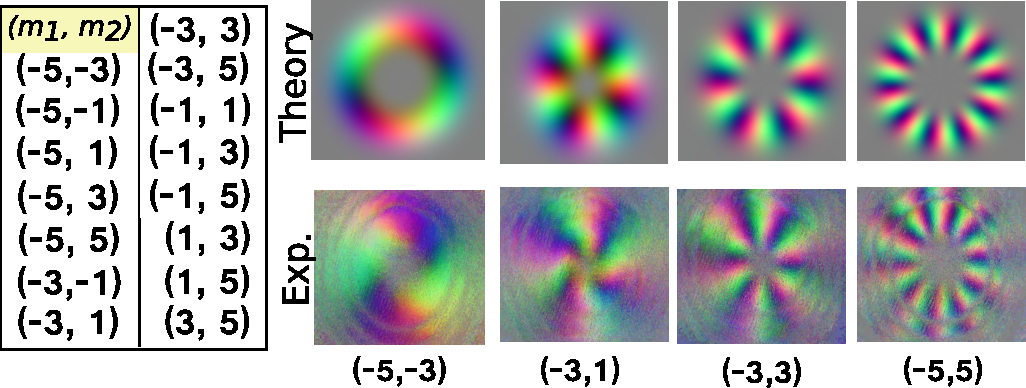
\includegraphics[width=0.7\textwidth]{VVBs-classification_with_CNN_schematics.pdf}
    \caption{
    	Comparison between simulated and experimental polarisation patterns for a sample of \acp{VVB}.
    }%
    \label{fig:VVBs:simVsExp}
\end{figure}



\section{Convolutional neural networks}
\label{sec:VVBs:CNNs}

\tmpHeading{What do we use CNNs for?}
We showcase the potential of \acp{CNN} to characterise experimentally generated states.
In particular, we test CNNs on two separate classification tasks:
finding the OAM numbers $(m_1,m_2)$ corresponding to input VVBs, and, assuming a dataset of VVBs with fixed $(m_1,m_2)$, finding the values of $(\theta,\phi)$ characterising each VVB image.

\tmpHeading{What are CNNs?}
\acp{CNN} are translation-invariant deep NNs designed to handle image classification tasks~\cite{lecun2015deep}. Among their countless applications, CNNs have been used to recognise off-centre images and segmented handwritten digits~\cite{simard2003best,ciresan2011flexible},
and for facial recognition tasks~\cite{matsugu2003subject}.
In its simplest form, a \ac{CNN} consists of a \emph{convolutional layer},
 % which consists of a series of nonlinear transformations applied to the input images,
followed by a \emph{max-pooling layer}, and finally a \emph{fully connected layer}.
These build up a mapping from each image to one of a finite number of output \emph{classes} defining the problem under consideration. In our case, the classes would be the $(m_1,m_2)$ pairs.
More precisely, the different layers operate as follows:
\begin{itemize}
	\item (\textbf{\emph{Convolutional layer}})
		The idea of the convolutional layer is to extract local features from the image.
		This is done by computing the inner product of every $k\times k$ block of the image with a fixed $k\times k$ matrix, referred to as a \emph{filter} in this context. The filter is applied sequentially to each $k\times k$ block of the image.
		% The size of these steps is known as the \emph{stride}. A stride of $1$ corresponds to the filter being applied to every single $k\times k$ contiguous block of the input.
		% Larger strides mean that some blocks are skipped.
		Each such filter extracts a specific feature from the image. The output of this process is called a \emph{feature map}. Multiple filters, and thus multiple feature maps, can be applied to the same image, to extract different features.
		The values of the filters, as well as the weights and biases of their connections with their input, are parameters to be trained.
		If the input images have dimensions $n_{ch}\times N_x\times N_y$, with $N_x,N_y$ width and height and $n_{ch}$ the number of \emph{channels} of the image (\emph{e.g.} $n_{ch}=3$ for RGB images), then a convolutional layer with $N_c$ filters will produce an output of size $N_c\times N_x\times N_y$.
		Convolutional layers are typically followed by a nonlinear function, applied elementwise to the outputs. A common choice is the so-called Rectified Linear Unit (ReLU), defined as $x\mapsto\max(x,0)$.
		This nonlinearity is crucial, lest the whole process be linear and thus unable to capture interesting features.
		Explicitly, we write each input image as a three-index tensor $\calI_{\alpha,ij}\equiv\calI^\alpha_{ij}$, with $\alpha=1,2,3$ the colour channels and $i,j=1,...,128$ indexing the pixels.
		Writing the filters as the tensor $\calF_{k\alpha mn}\equiv\calF^{k\alpha}_{mn}$, with $k=1,..,32$ indexing the different filters, we then compute the activation maps $\calM_{k\alpha pq}$ as
		\begin{equation}
			\calM_{k\alpha pq} = (\calF^{k\alpha}\star\calI^{\alpha})_{pq} \equiv
			\sum_{mn} \calF^{k\alpha}_{mn} \calI^\alpha_{R[p,q]_{mn}},
		\end{equation}
		where $\star$ denotes the $2$D convolution operation, which consists in computing the inner product of $\calF^{k\alpha}$ with the different $3\times3$ blocks of $\calI^\alpha$. Here, $R[p,q]$ denotes the indices of a $3\times3$ block surrounding the indices $p,q$.
		Explicitly, $R[p,q]_{mn}\equiv (p+m-2,q+n-2)$ with $m,n=1,2,3$, so that for example $R[1,1]$ covers the $3\times3$ submatrix surrounding the $(1,1)$ element of the image (which is the upper-left pixel). Whenever $R[p,q]$ covers pixels that fall outside of the boundaries of the image, like is the case for $R[1,1]$, it is standard practice to apply some \emph{padding} to the image, which in this case amounts to adding a single row or column of zeros on each side of the image. This is done to avoid having the bordering pixels being given a lesser weight than the rest.
		Once the activation maps are computed, the ReLU activation function is applied element-wise to $\calM_{k\alpha pq}$.
		This process is also illustrated in~\cref{fig:VVBs:convolutions_example}.
	\item (\textbf{\emph{Pooling layer}})
		After convolution and nonlinearity follows a \emph{max pooling} stage. Here, the feature maps are down-sampled, for example by subdividing each feature map into $\ell\times \ell$ blocks, and mapping each such block into its average value.
		This is used to filter out the most relevant features from the feature maps, thus reducing noise and increasing the efficiency of training.
	\item (\textbf{\emph{Fully connected layer}})
		Finally, a fully connected layer is applied to the output of the max-pooling stage, mapping its output to one of the different classes defining the problem.
		This stage operates like a standard NN layer.
		This is the layer at which the final decision is reached: based on the activations of the final neurons in this layer, the network takes a decision as to which class the input belongs to (for example by choosing the neuron with the largest activation).
\end{itemize}
Note that this is only the most basic structure found in CNNs. Actual CNNs will often contain different numbers of convolutional, pooling, and fully connected layers in different arrangements and with different parameters, depending on the specific applications.

\tmpHeading{How do we implement the CNN?}
To build and train the \acp{CNN} we use the Python library \emph{Keras}~\cite{chollet2015keras}.

% channel1 = ConstantArray[0, {7, 7}];
% channel1[[2 ;; 6, 2 ;; 6]] = RandomInteger[{0, 2}, {5, 5}];
% channel2 = ConstantArray[0, {7, 7}];
% channel2[[2 ;; 6, 2 ;; 6]] = RandomInteger[{0, 2}, {5, 5}];
% channel3 = ConstantArray[0, {7, 7}];
% channel3[[2 ;; 6, 2 ;; 6]] = RandomInteger[{0, 2}, {5, 5}];

% filter1 = RandomInteger[{-1, 1}, {3, 3}];
% filter2 = RandomInteger[{-1, 1}, {3, 3}];
% filter3 = RandomInteger[{-1, 1}, {3, 3}];

% grayBorderingSquares[size_Integer] := {LightGray,
%      Rectangle[{#1, #2} - 0.45, {#1, #2} + 0.45] &[##]
%      } & @@@ Select[
%     Tuples[Range@size, {2}],
%     Min@# == 1 || Max@# == size &
%     ];
% greenInsideSquares[size_Integer] := {LightGreen,
%      Rectangle[{#1, #2} - 0.45, {#1, #2} + 0.45] &[##]
%      } & @@@ Select[
%     Tuples[Range@7, {2}],
%     Min@# > 1 && Max@# < size &
%     ];
% squaresGrid[xs_, ys_, color_] := {color,
%    Rectangle[{#[[1]], #[[2]]} - 0.45, {#[[1]], #[[2]]} + 0.45] & /@ 
%     Tuples@{xs, ys}
%    };

% numbersInMatrix[matrix_] := Table[
%    Text[matrix[[Dimensions[matrix][[2]] + 1 - j, i]], {i, j}],
%    {i, 1, Dimensions[matrix][[1]]}, {j, 1, Dimensions[matrix][[2]]}
%    ];

% tripleCopy[expr_, size_] := 
%   Translate[expr, {0, #}] & /@ {0, -size - 1, -2 size - 2};

% fig = With[{size = Length@channel1}, Graphics[{
%     {grayBorderingSquares@size, greenInsideSquares@size} // 
%      tripleCopy[#, size] &,
%     Translate[numbersInMatrix@#[[1]], {0, #[[2]]}] & /@ Thread@{
%        {channel1, channel2, channel3}, {0, -size - 1, -2 size - 2}
%        }
%     (*{FaceForm[],EdgeForm[{Thick,Red}],Rectangle[{#2,
%     size+1-#1}-0.45,{#2,size+1-#1}+0.45]&[1,3]}*)
%     , 
%     tripleCopy[#, size] &@
%      {FaceForm[], EdgeForm[{Thickness@0.01, Red}], 
%       Rectangle[{5, 5} - 0.48, {7, 7} + 0.45] &[1, 3]},
%     Sequence @@ With[{xmin = 7, xmax = 12.5},
%       tripleCopy[#, size] &@
%        {Thick, Dashed, Red,
%         {Line@{{xmin, 4.5}, {xmax, 4.5}}},
%         {Line@{{xmin, 7.5}, {xmax, 7.5}}},
%         {Line@{{xmax - 3, 4.5}, {xmax - 3, 7.5}}},
%         {Line@{{xmax, 4.5}, {xmax, 7.5}}}}
%       ],
%     squaresGrid[Range[10, 12], Range[5, 7], LightRed] // 
%      tripleCopy[#, size] &,
%     Translate[numbersInMatrix[filter1], {9, 4}],
%     Translate[numbersInMatrix[filter2], {9, 4 - size - 1}],
%     Translate[numbersInMatrix[filter3], {9, 4 - 2 size - 2}],
%     Arrow@{{13, 6}, {15, 6}} // tripleCopy[#, size] &,
%     {FaceForm[], EdgeForm[{Black, Thick, Dashed}], 
%       Rectangle[{16, 6} - 0.5, {16, 6} + 0.5]} // 
%      tripleCopy[#, size] &,
%     Text[Style[
%       Total[Flatten@channel1[[;; 3, 5 ;; 7]]*Flatten@filter1], 
%       Bold], {16, 6}],
%     Text[Style[
%       Total[Flatten@channel2[[;; 3, 5 ;; 7]]*Flatten@filter2], 
%       Bold], {16, 6 - size - 1}],
%     Text[Style[
%       Total[Flatten@channel3[[;; 3, 5 ;; 7]]*Flatten@filter3], 
%       Bold], {16, 6 - 2 size - 2}]
%     }, ImageSize -> 300]]

\begin{figure}[tb]
    \centering
    \includegraphics[width=0.5\linewidth]{VVBs-CNNconvolutions-scheme-1row}
    \caption{
    	Simple illustration of how a filter is applied to an input image.
    	The green square represents an input image, focussing on a single channel. In our notation, assuming the first channel, this would be $(\calI^1_{ij})_{ij}$ with $i,j=1,...,5$.
    	The gray squares represent the padding applied to the image.
    	The dashed red square is a $3\times 3$ filter, which is here shown applied to the upper-right $3\times3$ block of the image.
    	In our notation, the filter is $\calF^{1,1}$ (assuming $k=1$ for the first filter). The thick red square is $R[1,5]$. The dashed black rectangle on the right contains the result of computing the inner product of the filter with the highlighted block of the image.
    	Being the result $1>0$, the ReLU nonlinearity leaves it unchanged.
    }%
    \label{fig:VVBs:convolutions_example}
\end{figure}

\tmpHeading{Categorisation into discrete classes}
We first feed the network with a training dataset of simulated \acp{VVB}. The goal is to classify states in $15$ classes, each one defined by a pair of OAM numbers $(m_1,m_2)$, as per~\cref{fig:VVBs:simVsExp}.
For each class we generate states with $\theta=\pi/2$ and $\phi\in[0,2\pi]$. The size of the training set is $400$ images per class.
% Additional $100$ simulated images per class are used to benchmark the performance during training. In these conditions, the network achieves an accuracy of $100\%$.
We then collect $100$ experimental images per class, to use as test set.
To test the effectiveness of using simulated images to classify experimental ones, we add different fractions of experimental images into the training dataset.
\Cref{fig:VVBs:simVsExp} shows the mean accuracy per class against the fraction of experimental images added to the training dataset.
Remarkably, a small increase of the number of experimental images in the training set results in a good accuracy reached by the network: $12.5\%$ is already sufficient to achieve an average accuracy of $\sim 0.989$.


\tmpHeading{Retrieving the position in the Poincaré sphere}
We also test the network on a different problem: assuming $(m_1,m_2)$ is fixed, retrieve the parameters $(\theta,\phi)$ characterising the VVB (remembering the definition of VVBs as given in~\cref{eq:VVBs:definition_VVBs_field}).
In particular, we train a CNN to retrieve the values $(\theta,\phi)$ characterising VVBs corresponding to the OAM quantum numbers $m_1=-m_2=1$.
The network is thus trained to discriminate both rotations in the polarisation patterns (corresponding to changes of $\phi$), and variations in the colour tone (corresponding to changes of $\theta$).
To frame this as a classification task, we partition the sphere in $26$ disjoint sectors.
Working in spherical coordinates, we partition $\theta$ is in the $3$ intervals $\left[k \frac{\pi}{8}, (k+2) \frac{\pi}{8}\right]$ with $k=1,3,5$, and $\phi$ in the $8$ intervals $\left[t \frac{\pi}{4}, (t+1) \frac{\pi}{4}\right]$ with $t \in \{0,...,7\}$.
This leaves two classes surrounding the two poles of the sphere, corresponding to $\theta \in \left[0, \frac{\pi}{8}\right]$ and $\theta\in\left[ \frac{7}{8} \pi, \pi\right]$.
Partitioning makes the classification of VVBs closer to the border of two sectors harder, but nonetheless provides useful information about the suitability of CNNs for this kind of task.
We train the CNN with $500$ simulated images per class in the training set, and $125$ per class in the validation one. The maximum accuracy  achieved is $\sim 0.90$.
The suboptimality of this result can be understood as consequence of framing the problem as a classification task. Training a CNN for the corresponding regression task will potentially give much better results.


\section{Dimensionality reduction}
\label{sec:VVBs:dimensionality_reduction}

\tmpHeading{A different approach to classify images}
While CNNs provide good performance for general image classification tasks, the specific structure of the datasets we deal with can be leveraged to make for more efficient algorithms. In particular, we know that the datasets consist of intensity patterns associated with (mostly pure) quantum states.
% we can hope to achieve similar performances in the tasks we are interested in by exploiting additional structure that we know is intrinsic to our dataset, due to it consisting of a set of intensities associated with states of light.
In this section we present alternative approaches to extract information the dataset of interest, using \ac{DR} to expose the intrinsic structure of the dataset.


\tmpHeading{DR and PCA}
\acf{DR} is a class of algorithms whose goal is to find low-dimensional encodings of high-dimensional datasets~\cite{cunningham2008dimension,fodor2002survey}.
This has several applications, from data visualisation, to improving the efficiency of classification and regression algorithms, which can be applied on the reduced representation of the data.
A classical \ac{DR} algorithm is \acf{PCA}.
In its simplest form, \ac{PCA} is a \emph{linear} \ac{DR} algorithm which, given a dataset of vectors in a high-dimensional space $\RR^n$, finds the directions which capture the maximum amount of information about the dataset~\cite{jolliffe2011principal,jolliffe2016principal}.
More specifically, given a dataset comprised of $N$ real vectors of length $M$, we define the \emph{data matrix} $\bs X$ as the $N\times M$ matrix whose $i$-th row is the $i$-th dataset vector. \ac{PCA} then finds the vectors $\bs a\in\RR^{M}$ that maximise the variance of $\bs X\bs a$. This turns out to be equivalent to diagonalising $\bs S\equiv \tilde{\bs X}^T\tilde{\bs X}/(N-1)$, where $\tilde{\bs X}$ is the \emph{centered data matrix}, which is equal to $\bs X$ modulo each of its columns shifted in order to average to zero.
The first $k$ \emph{principal components} found by \ac{PCA} are then the $k$ eigenvectors of $\bs S$ corresponding to the largest $k$ eigenvalues.
Note that these principal components are themselves vectors of the same ``type'' as the data vectors. This means that \ac{PCA} effectively generates a set of data vectors which ``optimally represent'' the information content of the given dataset.

\tmpHeading{PCA and VVBs}
The rationale behind using \ac{PCA} in the context of \acp{VVB} is that, although experimental images live in extremely high-dimensional spaces (whose dimension is of the order of the number of pixels of the \ac{CCD} camera), the underlying dimension of the generated \acp{VVB} is typically much lower.
This means that, although the experimental dataset might \emph{a priori} seem like a complicated bundle of high-dimensional vectors, the underlying data is actually characterizable by a small number of parameters.
% Furthermore, the linearity of the mapping from the full to the reduced space makes it preserve many of its geometrical properties.
This is a form of \emph{unsupervised} learning, in that we gain useful information about the the images without feeding the algorithm with any prior knowledge about their structure.


% \tmpHeading{For example...}
% For example, in our case, each row of $\bs X$ is a vector of length $128\times128\times3$ containing the Stokes parameters $S_{b_1}, S_{b_2}, S_{b_3}$ for each pixel of the camera.
% Because each image corresponds to such a vector, and vice versa each such vector corresponds to the image of a \ac{VVB}, we can represent the principal components found by \ac{PCA} again in the form of images, which allows us to gain some intuition into the type of principal components that optimally represent the data according to \ac{PCA}.


\subsection{Retrieving states from probabilities}

\tmpHeading{Measuring in a single measurement basis}
Collecting experimental intensity images with the \ac{CCD} camera is akin to measuring output probabilities in a fixed measurement basis.
In general, this is not sufficient to fully reconstruct a state.
However, specific conditions (such as sparsity of the state and an appropriate choice of measurement basis) still allow for a full reconstruction~\cite{banchi2018multiphoton}.
More specifically, let $\rho$ be the density matrix characterising a state, and let us assume that this state is low-rank (that is, only a small number $n$ of eigenvalues of $\rho$ are non-vanishing).
The output probabilities in the computational basis following evolution through a unitary $\calU$ are
\begin{equation}
	p_k = (\calU\rho\calU^\dagger)_{kk}
	    = \sum_{ij}\calU_{ki}\bar\calU_{kj}\rho_{ij}.
\end{equation}
% Note that this situation models what happens when we measure VVBs with a CCD camera: VVBs are sparse in the OAM-polarisation basis (they are effectively two-dimensional), and measurement in the position basis can be described as a projective measurement following a unitary $\calU$ describing the change of basis.
This means that the mapping between density matrices and detected probabilities is linear: $\bs p=\Psi(\rho)$ for some linear map $\Psi$.
We can represent $\Psi$ as a (generally non-square) matrix, for example via its action on the coefficients of $\rho$ in some operatorial basis.
Given $\rho=\sum_k c_k \sigma_k$ for some basis $\{\sigma_k\}_k$ of traceless Hermitians, we have the induced linear mapping $p_j = \sum_k \Psi_{jk}c_k$, with $\Psi_{jk}\equiv\Psi(\sigma_k)_j$ the matrix elements of $\Psi$.
This linearity implies that many geometrical features of the space of states are preserved in the space of probabilities. Moreover, a suitable choice of $\Psi$ will allow to retrieve $\rho$ from the knowledge of $\bs p$.
For this to be possible, $\Psi$ needs to have a number of rows greater than or equal to the number of columns. Physically, this amounts to the measurement basis containing a sufficient number of elements. More specifically, $\Psi$ needs to be \emph{left-invertible}, which is the case when its columns are linearly independent.

\tmpHeading{Application to experimental VVB images}
In our case, $\rho$ is a description of a VVB in the OAM-polarisation basis, which is the basis in which it is sparse, while $\calU$ is the unitary mapping this basis into the position basis, which is the one that CCD cameras naturally operate on. In principle, one might need to take care of the different dimensionality of these spaces (the OAM space is countable while the position one is not), but this is easily fixed by discretising the position space, which is what is done naturally by the finite number of pixels of the CCD camera. 
The set of detected probabilities is then given by $\bs p=\on{diag}(\calU\rho\calU^\dagger)\equiv\Psi(\rho)$.
Crucially, the linearity of $\Psi$ implies that it preserves the \emph{convexity} of the space of states.
For example, if we consider the set of states of the form $c_0 \ket{\uparrow,m=m_1} + c_1 \ket{\downarrow,m=m_2}$ with $m_1\neq m_2$, the corresponding density matrices will be arranged to form a three-dimensional sphere embedded in the full state space (because these are effectively different states of a single qubit).
Thanks to the linearity of $\Psi$, \emph{the corresponding probabilities $\bs p$ will also be contained in a spherical surface}, up to possible rescaling of the axes.
In other words, the Bloch sphere of the original two-dimensional system is still present, albeit hidden, in the experimental images, embedded into an extremely high-dimensional space.


\begin{figure}[tb]
    \centering
    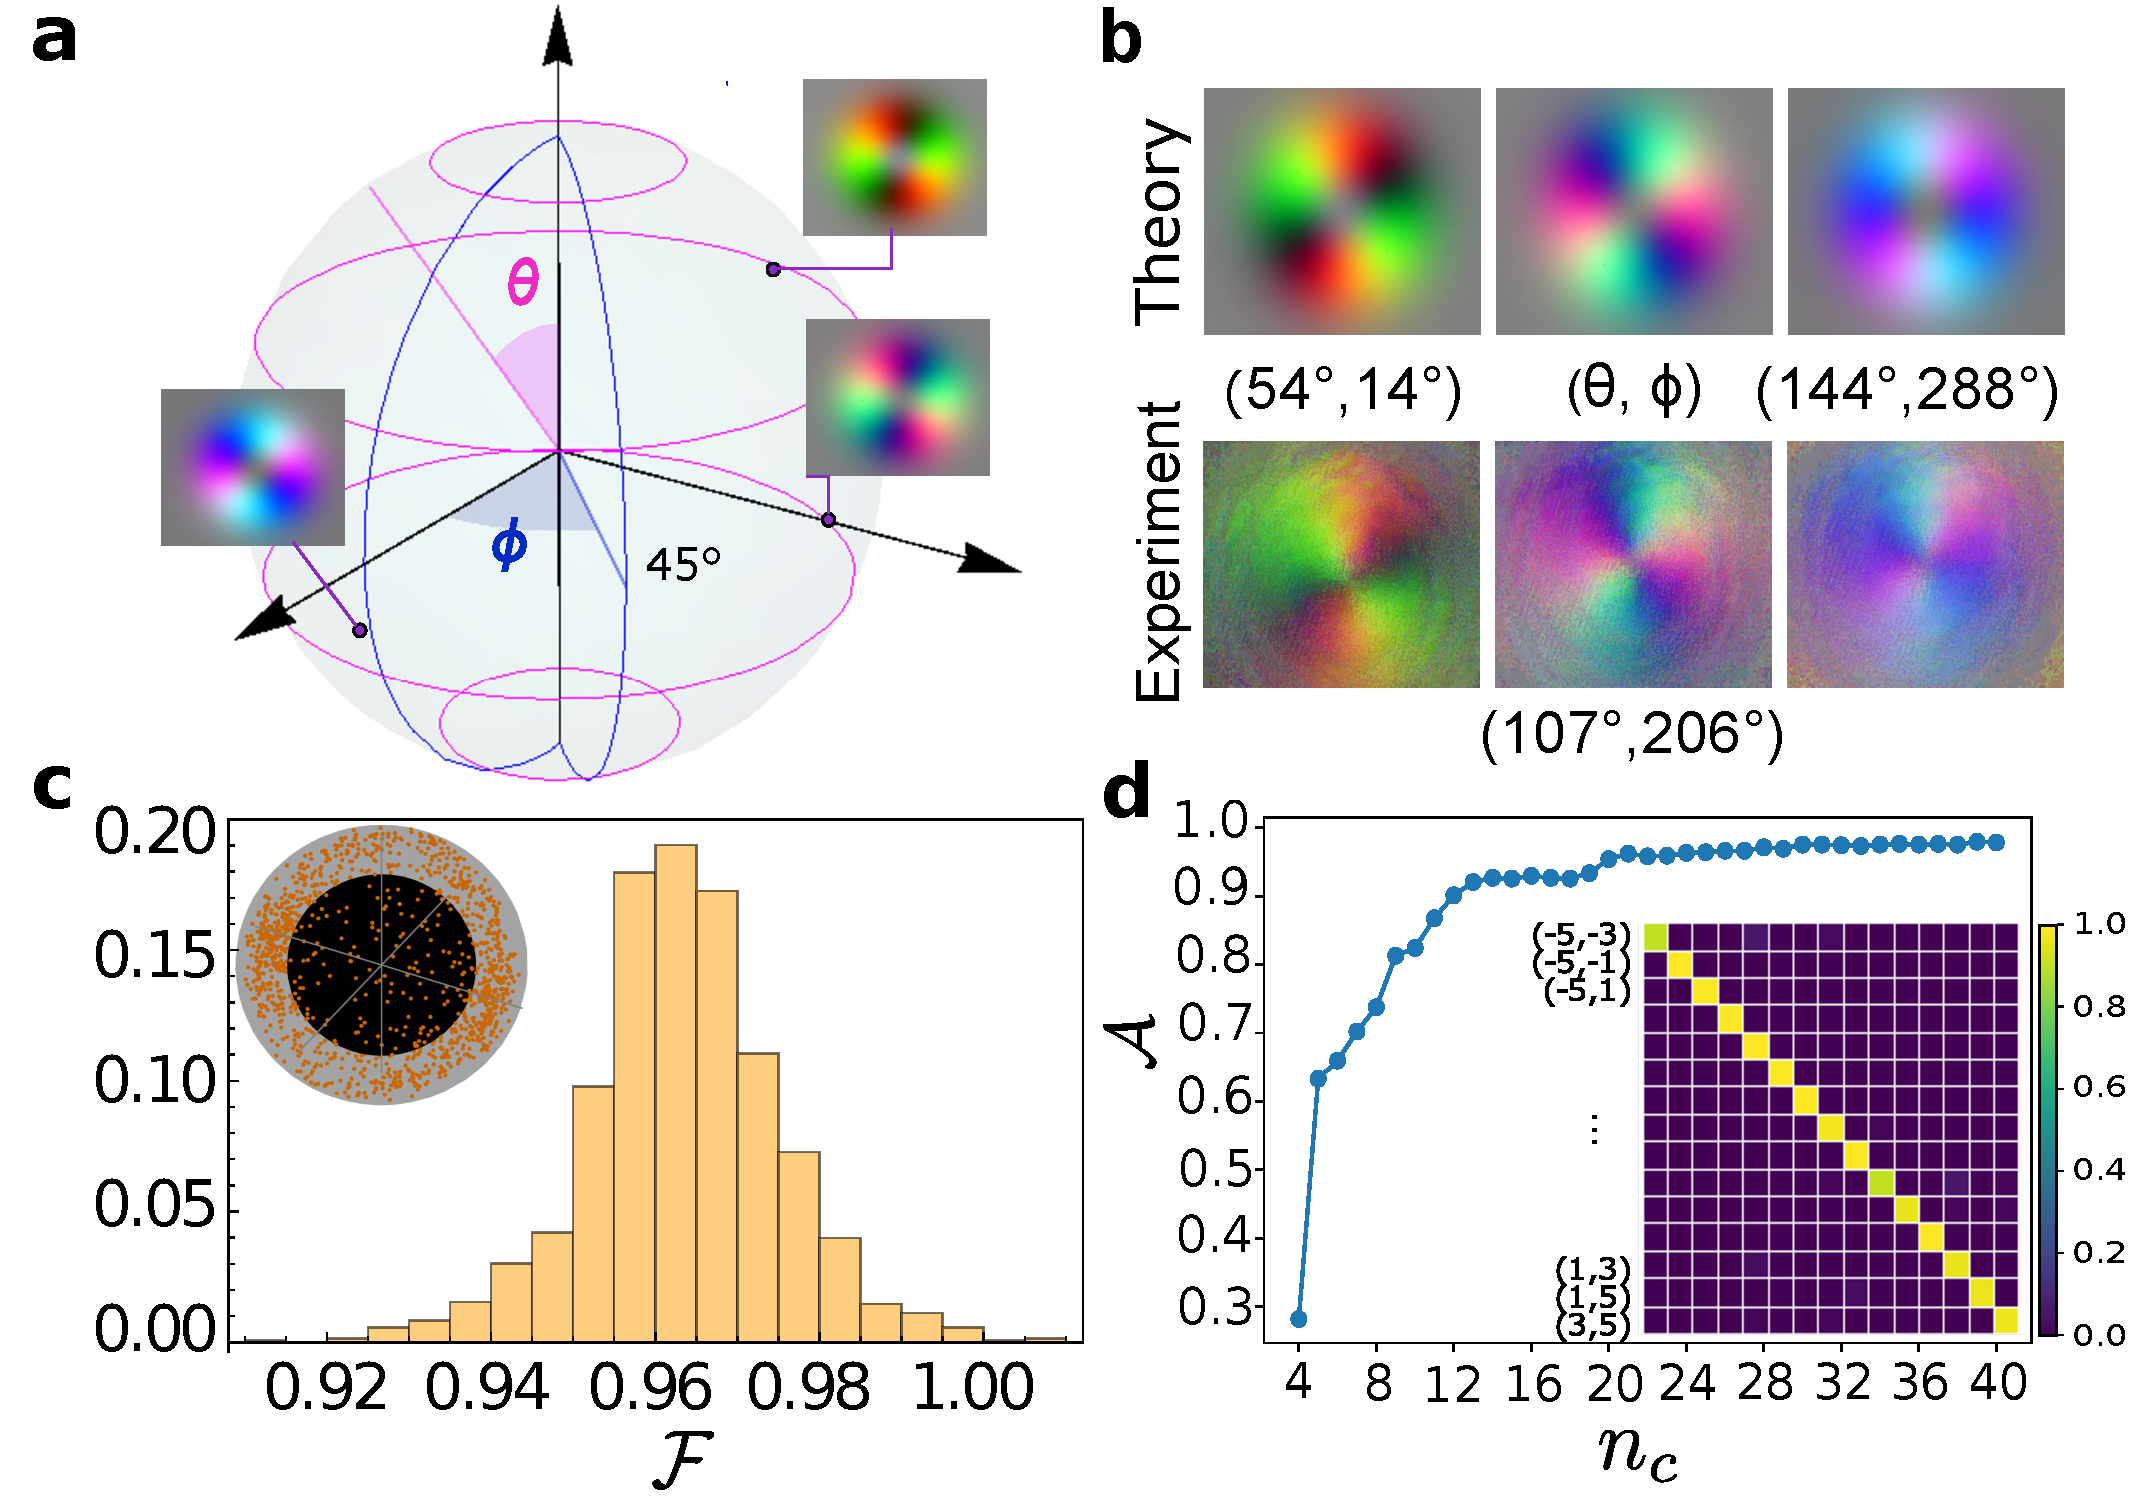
\includegraphics[width=0.8\linewidth]{VVBs-Fig4.pdf}
    \caption{
		\textbf{(a)} High order Poincar\'e sphere for \acp{VVB} with $|m_{1,2}|=1$. Magenta-coloured parallels (Blue-coloured meridians) mark intervals between consecutive values of $\theta$ ($\phi$). 
		Along a meridian the colours of the pattern vary from the hottest to the coldest one. Along a parallel, the patterns rotate.
		\textbf{(b)}
		Comparison between experimental and simulated \ac{VVB} images for different angles $(\theta, \phi)$.
		\textbf{(c)}
		Distribution of fidelities obtained comparing each experimental VVBs with its reduced 3D representations given by PCA. Projecting each image onto its first three principal axes and rescaling brings the data (orange points) onto a sphere in 3D, as shown in the inset. The inner (outer) black (semi-transparent) sphere is added for contrast [radius equal to that of the point with smaller (larger) radius]. \highlight{togliere la sfera}
		\textbf{(d)}
		Average prediction accuracy of a linear \ac{SVM} classifier, trained and tested after applying linear DR to the data, against the number of reduced dimensions $n_c$.
		For each of the 15 classes (cf.~\cref{fig:VVBs:simVsExp}) in which the experimental dataset was divided, we show in the inset the true-table. 
    }%
    \label{fig:VVBs:PCAresults}
\end{figure}


\subsection{Results}

\tmpHeading{PCA applied to experimental data}
As a notable example, we apply these observations to VVBs with $m_2=-m_1=1$.
These are the states of the form $c_0 \ket{L,m=1} + c_1 \ket{R, m=-1}$ with $\abs{c_0}^2+|c_1|^2=1$.
We find that applying PCA to a dataset of images corresponding to these VVBs naturally produces the underlying Bloch sphere representation:
the first three singular values are sufficient to capture most of the information, and projecting the images along the corresponding axes, the dataset is in good approximation arranged on a three-dimensional sphere.
Note that is not a straightforwardly deduced from the experimental images alone, but is easily found via \ac{DR}.
This result highlights the potential of \ac{DR} to reveal features of the states generating a given experimental dataset, also in the presence of experimental noisy conditions.
To assess the accuracy of such reconstruction, we compute the average fidelity $\calF_{\on{avg}}$ between the expected state and the one found by our analysis with PCA.
This is found to be $\calF_{\on{avg}}\sim0.96$, with standard deviation $\sim0.01$, thus certifying the quality of the reconstruction.
The full histogram of fidelities is given in~\cref{fig:VVBs:PCAresults}\textbf{c}, 

\begin{figure}[tb]
  \centering
  \includegraphics[width=0.98\textwidth]{S1_fig.png}
  \caption{
      \textbf{a,}
       Principal components obtained using PCA on simulated datasets of noisy VVB. The first (second) row shows the first seven principal components obtained on the dataset $\mathcal S_1$ ($\mathcal S_2$). 
       The first 6 (all 7) components correspond to non-vanishing singular values.
       \textbf{b,} First 40 principal components individuated in the experimental dataset corresponding to the 15 classes labelled by $(m_1,m_2)$, discussed in the main text.%
    }
    \label{fig:VVBs:principal_components}
\end{figure}


\tmpHeading{Toy examples of application of PCA to VVBs}
To illustrate the usefulness of these ideas in understanding the type of states generated by a given apparatus, we consider here two additional examples of \ac{PCA} applied to different types of input states. 
% In all of these cases, \ac{PCA} is applied without any previous knowledge of the type of states that underlie the observed experimental images, and is therefore to be considered a type of \emph{unsupervised learning}.
Consider a set of simulated images corresponding to VVBs of the form
$c_1\ket{L,m=1}+c_2\ket{R,m=2}$ and
$c_1\ket{L,m=1}+c_2\ket{R,m=4}$, where the coefficients $c_i$ are sampled uniformly at random from the set of $c_{1},c_2\in\mathbb{C}$  such that $|c_1|^2+|c_2|^2=1$.
Applying PCA to this dataset, we find six non-vanishing singular values, whose associated principal components are given in~\cref{fig:VVBs:principal_components}\textbf{a}.
This is consistent with the dimension of the subspace  spanned by the states in $\calS_1\equiv\{c_1\ket{L,1}+c_2\ket{R,2}, c_3\ket{L,1}+c_4\ket{R,4}\}$,  as the set of corresponding density matrices is spanned by the six orthogonal matrices
$X^{(1,2)}, X^{(1,4)}, Y^{(1,2)},Y^{(1,4)},Z^{(1,2)}\pm Z^{(1,4)}$, where $X^{(i,j)}=\ketbra{i}{j}+\ketbra{j}{i}$ is the Pauli $X$ matrix acting on the $(i,j)$ subspace, and $Y^{(i,j)}$ and $Z^{(i,j)}$ are similarly defined.
On the other hand, if the dataset under consideration consists of states in the space $\mathcal S_2=\{c_1\ket{L,1}+c_2\ket{R,2}, c_3\ket{L,3}+c_4\ket{R,4}\}$, then \ac{PCA} finds \emph{seven} principal components associated with non-vanishing singular values, as again shown in~\cref{fig:VVBs:principal_components}\textbf{a}.
This is consistent with the underlying state space being spanned by the seven orthogonal Hermitians:
\begin{equation}
\begin{gathered}
    X^{(1,2)}, \,\, X^{(3,4)}, \,\,
    Y^{(1,2)}, \,\, Y^{(3,4)}, \\
    Z^{(1,2)},\quad
    -Z^{(1,2)} + 2 Z^{(1,3)}, \\
    -Z^{(1,2)} - Z^{(1,3)} + 3 Z^{(1,4)}.
\end{gathered}
\end{equation}
These matrices can be derived by direct analysis by finding a set of orthogonal Hermitians generating the set of density matrices in $\calS_2$.
This method thus provides a quick and easy way to obtain useful information about the dimensionality of generated states, as well as about other properties such as specific symmetries, which, as shown in~\cref{fig:VVBs:principal_components}, are often picked up by the principal components.


\section{Support vector machines}
\label{sec:VVBs:SVMs}


\tmpHeading{What are SVMs?}
\acfp{SVM} are a class of \emph{supervised learning} algorithms, whose goal is to classify data into discrete classes. \acp{SVM} work by finding a partition of the feature space such that all the vectors with the same training label lie on the same classification sector.
In particular, \emph{linear} \acp{SVM} look for an optimal \emph{linear} partition of the data.
As supervised learning algorithms, SVMs take as input a training set of labelled data of the form $\{(\bs x_1,\ell_1),...,(\bs x_n,\ell_n)\}$, where $\bs x_i\in\RR^N$ and $\ell_i$ is one of two possible labels. If there are only two possible labels, we conventionally assume $\ell_i\in\{-1,1\}$.
A linear separation is characterised by two parameters $\bs w$ and $b$, which identify an hyperplane as the set of $\bs x\in\RR^N$ such that $\bs w\cdot\bs x=\bs b$. We want this hyperplane to be such that, for all training vectors $\bs x_i$, the constraint
\begin{equation}
	\ell_i(\bs w\cdot\bs x_i-\bs b)\ge1
	\label{eq:VVBs:SVMs_basic_condition}
\end{equation}
is satisfied. This would imply that all (and only the) $\bs x_i$ corresponding to $\ell_i=1$ lie on the same side of the hyperplane.
New data is then categorised using the \emph{classifier} $g_{\bs w,\bs b}(\bs x)=2\Theta(\bs w\cdot\bs x-\bs b)-1$, which equals $\pm1$ depending on whether the point $\bs x$ is on one side of the separation or the other.
The constraint in~\cref{eq:VVBs:SVMs_basic_condition} identifies the so-called \emph{hard-margin} SVM, because this is only possible if every single training point is strictly on one or the other side of the separating hyperplane.
An often more practical alternative are the so-called \emph{soft-margin} SVMs, in which this strictness is lifted. Instead, the goal becomes to minimise the average value of
$\max(0, 1- \ell_i (\bs w\cdot\bs x_i-\bs b))$, trying at the same time to keep $\|\bs w\|$ as low as possible. This variation makes the algorithm more robust and able to classify data even in the presence of some noise.

\tmpHeading{SVMs after PCA}
We now show how the reduced representations provided by \ac{PCA} can function as starting point to train a classifier with an accuracy comparable with that of the \acp{CNN} used in~\cref{sec:VVBs:CNNs}, whilst requiring a drastically reduced amount of computational resources.
More precisely, we use as classifiers linear multiclass \acp{SVM}~\cite{hearst1998support,shawe2000support}.
Both training and classification are performed \emph{after} the dimensionality reduction has been carried out via \ac{PCA}. This makes for improved computational times as well as making the algorithm more robust to experimental noise and imperfections.
As done for the \ac{CNN}, we consider the task of classifying experimentally generated VVBs. We train a \ac{SVM} on the reduced space obtained via \ac{PCA}, for the task of categorising images according to their OAM quantum numbers $(m_1,m_2)$.
What's more, the geometrical picture offered by the reduced representation tells us when we should expect this classification to be accurate: \ac{PCA} effectively retrieves the description of the states in the generalised Bloch representation, therefore the classification will give good results whenever the states are linearly separated in state space.

\tmpHeading{Results}
We use half of the dataset for training, and the other half for testing the resulting accuracy.
We found a \emph{linear} SVM, instead of a more commonly employed SVM with RBF kernel, to give better accuracies: $\sim98\%$ vs the $\sim94\%$ using the RBF kernel.
In~\cref{fig:VVBs:PCAresults}\textbf{d}, we highlight how the average overall accuracy depends on the dimension of the reduced representation: $\sim 25$ dimensions are already sufficient for good accuracies.
A breakdown of the classification performance is reported in~\cref{fig:VVBs:accuracies15classes_SVC}.
The average classification accuracy is $\sim 98 \%$. This result confirms that the description provided by \ac{PCA} is sufficient to capture the important features of the generated states, thus allowing for significantly more efficient classification schemes.

\begin{figure}[tb]
  \centering
  \includegraphics[width=0.7\textwidth]{Figures/VVBs/VVBs-svcAccuracies_15classes_halftrainingdata_40dims_usedInPaper.pdf}
  % \includegraphics[width=0.9\textwidth]{Figures/VVBs/VVBs-svcAccuracies_15classes_halftrainingdata_40dims_linear.pdf}
  \caption{
      Classification accuracies given by the SVM classifier used on the reduced dataset obtained via PCA.
      \highlight{aggiornare figura, mettere quelle dal paper}
    }
    \label{fig:VVBs:accuracies15classes_SVC}
\end{figure}

\begin{figure}[tb]
  \centering
  \includegraphics[width=0.7\textwidth]{Figures/VVBs/VVBs-accuracies15classes_CNN2.pdf}
  % \includegraphics[width=0.9\textwidth]{Figures/VVBs/VVBs-svcAccuracies_15classes_halftrainingdata_40dims_linear.pdf}
  \caption{
      Classification accuracies given by the SVM classifier used on the reduced dataset obtained via CNN.
    }
    \label{fig:VVBs:accuracies15classes_CNN}
\end{figure}


\section{Conclusions}
\label{sec:VVBs:conclusions}

We presented a novel approach to classify \acp{VVB} leveraging ML techniques. We demonstrated how the use of inference strategies based on CNNs, PCA, and SVMs allows to extract efficiently properties of high-dimensional photonics \ac{VVB} systems.
In particular, we used DR to probe the underlying geometrical properties of experimentally generated VVBs, without requiring prior knowledge about the physics of the generation apparatus.
% By embedding a variety of \ac{ML} algorithms into our experimental pipeline, the task of characterising structured light is made significantly broader in the methods, ranging from supervised to unsupervised learning, and more flexible in the applications, classification and regression tasks.
%Then, the investigation of different techniques in the ML field has provided a more general framework for the characterization of structured light.  
% While paving the way for further experimental validations, potentially also in non-photonics settings, we believe that numerous tasks of relevance to modern photonics could benefit from introducing similar {\ac{ML}} ideas into their characterisation protocols.
The flexibility of the techniques we deployed makes the applicability of this type of  analysis extend to a variety of different experimental scenarios.
% These techniques can prove to be useful add-on to tasks ranging from the design of automatised approaches to the characterisation of experimental platforms and experiments, to the provision of solutions to OAM demultiplexing in the context of classical and quantum communication and, more generally, for the use of structured light in quantum technologies.


\chapter{Conclusions}
\label{chapter:conclusions}
We discussed the use of machine learning techniques to tackle different quantum information tasks.
On one hand, we showed that borrowing techniques from the machine learning toolbox, such as stochastic gradient descent and automatic differentiation, offers significant advantages for tasks such as gate learning with time-independent Hamiltonians.
Moreover, we found that pairing supervised learning strategies with analytical reasoning we can further speed-up finding solutions, and gain more insight into the structure of the problem.
On the other hand, after devising and showcasing experimentally a scheme to generate arbitrary states via quantum walk dynamics, we showed how machine learning algorithms such as convolutional neural networks, principal component analysis, and support vector machines, can provide significant insight into generated states from the sole knowledge of their transverse intensity profiles.
These results add to the growing amount of evidence that the flexibility provided by machine learning finds fruitful application both for fundamental and applied research in quantum information science.

The work presented in this thesis lends itself to be extended in several directions.
In the context of gate learning, there are three major venues of research branching from the results presented in~\cref{chapter:gate_learning}.
From a more applicative point of view, there is much to be learnt about what quantum gates are directly implementable with experimentally available interactions.
A thorough understanding of this would have far-reaching consequences for example in the context of quantum computation and quantum algorithms development, providing more expressive quantum gates to be included into the ``elementary gate set'' used to express quantum algorithms and decompose complex operations.
The underlying mathematical questions are also compelling and ripe for exploration. There are interesting relations between our methods and mathematical results in the fields of \emph{inverse eigenvalues problems}~\cite{friedland1977inverse} and Lie theory that could potentially provide elegant answers to the question of reachability of quantum gates in constrained interactions scenarios.
Another future venue of research is the extension of our analytical results for quantum gates to the more general context of quantum maps.
In particular, how the analytical conditions discussed in~\cref{chapter:gate_learning} would extend to the case of non-unitary evolutions.
Finally, the machine learning techniques we used in this work are intrinsically black-box-like algorithms.
Even though they are well-suited to gate learning problems, they are not intrinsically tied to them, and can be seamlessly applied to other contexts.
Indeed, any problem requiring to optimise \emph{a functional relationship} over a number of continuous parameters is likely to be a good candidate for the combination of the supervised learning techniques we employed.
A promising candidate would for example be finding convex decompositions for given classical states, for which a similar technique based on stochastic gradient descent would be potentially fruitful.

The results presented in~\cref{chapter:quantum_walks,chapter:experimental_engineering_qudits} are also of wide applicability.
The generality of our characterisation of the possible quantum states emerging from one-dimensional discrete-time quantum walks makes it potentially useful in any task involving a finite number of steps of such dynamics.
From an applicative perspective, the protocol allows the generation of arbitrary qudit states using only a simple physical interaction, as demonstrated in the experimental realisation presented in~\cref{chapter:experimental_engineering_qudits}.
Extending the result would contribute to a more thorough understanding of quantum walk dynamics, which are of widespread use in quantum information science and have found countless applications.
In particular, a natural open question is the extensibility of our characterisation to quantum walks on higher dimensional lattices, as well as quantum walks on general graphs.
More generally, a deeper understanding of the exact properties of quantum walk dynamics that make this characterisation possible in the first place would lead to generalise our results for a wide range of quantum dynamics even beyond the quantum walk model.

Finally, our application of machine learning to analyse experimentally generated states further showcases the usefulness and flexibility of these techniques in a multitude of scenarios.
These include, but are not limited to, any situation involving measuring high-dimensional quantum states in a fixed basis.
Possible extensions of this work include a more thorough analysis of vector vortex beams, and the use of more sophisticated models to describe the experimental outputs of q-plates.
On the machine learning side, a question left open by our investigation is the possibility of classifying accurately experimental vector vortex beams using convolutional neural networks trained exclusively on simulated ones.
Extending the techniques used in~\cref{whatever} to achieve this would provide an even stronger statement about the possibility of leveraging machine learning algorithms to devise automatic pipelines to characterise and validate the quality of experimental apparatuses in a variety of scenarios.
A first possible step in this direction would be to leveraging the recent developments in \emph{neural network interpretability}~\cite{olah2018the} to extract the features picked up by the trained neural networks. This would, in turn, allow to devise techniques making the generalisation from simulated to experimental images possible.


%!TEX root = ./Thesis.tex

\clearpage
\phantomsection
\addcontentsline{toc}{chapter}{Bibliography}

% \bibliographystyle{IEEEtran} % IEEE bibliographic/citation style.
% %\bibliography{IEEEabrv,Thesis}
% \bibliography{IEEEfull,Thesis}
\newrefcontext[sorting=nty]
\printbibliography



\end{document}
